
\chapter{Methods}
\label{methods}
Consider the case that we have a short recording of an unknown instrument playing, and we want a model that allows us to mimic this instrument with new melodies - that is, we are interested in few shot timbre transfer.
Using the baseline architecture, a model would need to be trained on the recordings of the new instrument, and then used to generate new melodies. An analysis of the capabilities and limitations of the baseline model is given in \Cref{baseline}.
In this thesis, the limits of fine-tuning a model to any new instruments are explored. However, before diving into transfer learning in \Cref{transfer}, some general improvements to the model are explored that yield an improved baseline. \newline
Using the first simple modification, the model can be forced to separate timbre from melody and perform one-shot timbre transfer for instruments it has seen during training.
This improvement relies on making $z$ constant over time, such that timbre transfer can be done by simply extracting $z$ of a recording of a target timbre, and feeding it to the decoder together with the $f_0$ and loudness curve of the target melody.
A more detailed analysis of this method follows in \Cref{time-constant-z}. \newline
The total amount of information available to the decoder is strongly limited through this modification, which hurts reconstruction accuracy but improves the disentanglement of melody and timbre. Other tweaks of the model, namely a bug fix of the algorithm that computes loudness and a modification of the multiscale-spectrogram loss make up for the drop in reconstruction accuracy and yield a model that can mimic diverse instruments such as flute, trumpet, violin, bass, guitar, sounds of the iconic Roland sh101 synthesizer and to some extend even various drums. \newline
Details on the datasets used are given in \Cref{datasets}. \newline



\section{Baseline architecture}
\label{baseline}
In order to encode the audio signal, loudness is computed using a rule-based algorithm with no trainable parameters as described by \citet{hantrakul_fast_2019-1}. The $f_0$ encoder is a pretrained convolutional neural network called CREPE that operates directly on the waveform, and the $z$-encoder consists of fully connected and GRU-layers \citep{chung_empirical_2014} working on mel-frequency cepstral coefficients (MFCCs) computed from the waveform. If the training data is collected from a single instrument, reconstruction is possible from only the pitch and loudness curves, without the need for a $z$-encoder. However, all models trained for this thesis use a $z$-encoder. All latent variables are time-distributed with a frame rate of 250 Hz, much below the sample rate of the waveform, which is 16000 Hz.\newline
The decoder controls two synthesizers: an additive harmonic synthesizer and a filtered noise synthesizer. The harmonic synthesizer gets $f_0$ directly as input and requires a time-varying amplitude distribution over 100 harmonics which is predicted by the decoder. \newline
The filtered noise synthesizer applies band-pass filters to white noise using 65 noise magnitudes at every time frame, which are also an output of the decoder.
Fully connected layers and one GRU layer are used in the decoder. \newline
If the model is trained on audios of a single instrument, e.g. a violin, the decoder interprets every melody as played by a violin and can therefore be used to perform timbre transfer.
However, if the model is trained on multiple instruments at once, it infers the timbre from the latent variable $z$. 


\subsection{Measuring Timbre Transfer Performance}
Evaluation of a model's capabilities to perform timbre transfer is often done by subjective listening tests.
In order to automatically evaluate a large number of models in a deterministic setup, I used a cycle-consistency inspired loss function.
To compute the loss, two timbre transfers are performed: a sample $a$, say a violin recording, is reconstructed by transferring its timbre onto an intermediate melody of a sample $b$, e.g. a melody extracted of someone singing.
The resulting audio is then used as a target timbre for the second timbre transfer, where the pitch and loudness of $a$ are used as the target melody to obtain $\hat{a}$.
Ideally, both synthesized audios should have different melodies but the timbre of the violin in $a$, and therefore $\hat{a}$ approximates $a$ and is called the cycle reconstruction of $a$. A schematic representation of the loss function is shown in \Cref{cycle-reconstruction}.

\begin{figure}
\centering
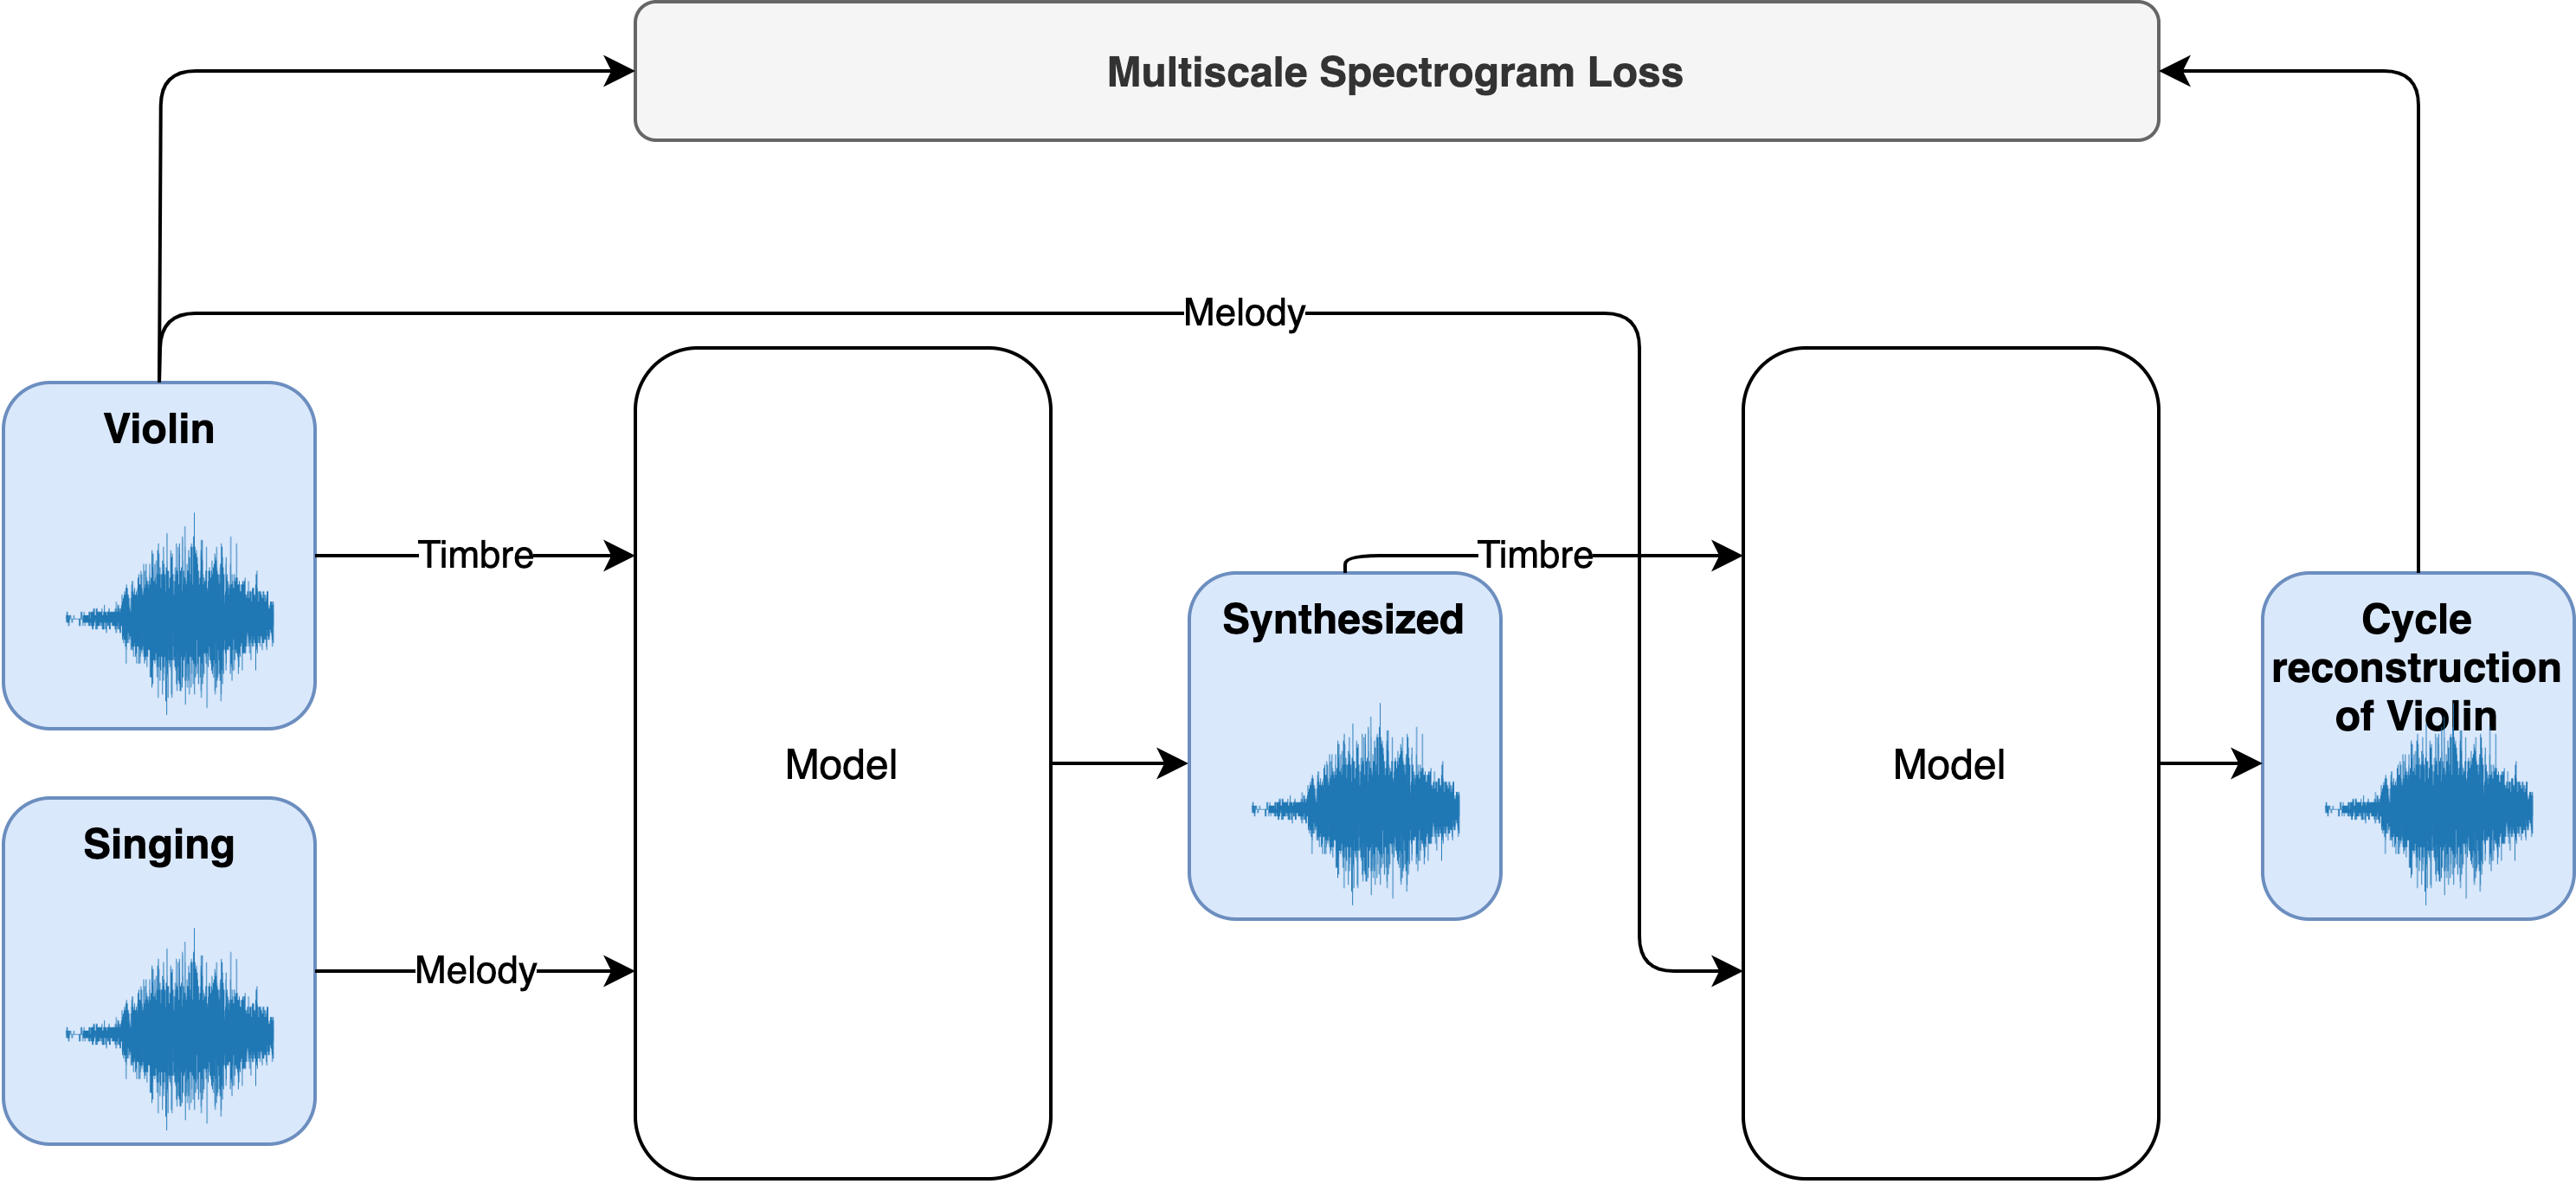
\includegraphics[width=0.8\textwidth]{figures/cycle_reconstruction_loss.png}
\caption{The cycle-reconstruction loss}
\label{cycle-reconstruction}
\end{figure}

A baseline model trained on monophonic recordings of the URMP dataset can reconstruct recordings of a held out test set consisting of the same instruments.
However, if we use the model to perform a timbre transfer, the audio sounds noisy and the timbre is barely recognizable, which is reflected by a poor cycle reconstruction loss. Error heatmaps of respective spectrograms are shown in \Cref{fig:cycle-reconstruction-error-exp1}.


\subsection{Datasets}
\label{datasets}
Multiple datasets with different instruments and varying total amounts of audio data serve as training data for the models, an overview is given in \Cref{table:datasets}.
The bass, guitar and drum datasets are published by the Frauenhofer IDMT institue \citep{idmt_bass} \cite{idmt_guitar} \citep{idmt_drum}.
The URMP dataset has been released by \citet{li_creating_2019} and contains a large number of different instruments. Some experiments for this thesis are performed only on the URMP dataset, while others are made on all listed datasets.
Last but not least, the sh101 dataset was kindly provided by Thomas Haferlach and is currently not published. \newline
Of each dataset, only the raw audio data of monophonic recordings is used for the experiments - none of the additional meta-data.
In particular have the models not been trained to explicitly classify the instrument of the audio, instead the timbre is modeled as a continuous latent vector with 16 dimensions.
The wavefiles were shuffled and split into training and test sets that remained fixed across all experiments.
In a preprocessing step, the audio was resampled to 16 kHz, loudness and pitch were computed and snippets of four seconds were extracted. \newline


\begin{table}
\begin{tabular}{lll}
\toprule
Dataset & Audio Data & Instruments \\
\midrule
bass\_train &   00:03:30 & \multirow{2}{*}{Bass} \\
bass\_test &   00:02:20 & \\
\hline
guitar\_train &   00:38:26 & \multirow{2}{*}{Guitar} \\
guitar\_test &   00:22:48 & \\
\hline
idmt\_drum\_train &   00:34:10 & \multirow{2}{*}{\shortstack[l]{Drum loops of acoustic drums, drum sample libraries and\\drum synthesizers}} \\
idmt\_drum\_test &   00:23:43 \\
\hline
sh101\_train &   00:48:43 & \multirow{2}{*}{Samples of a Roland sh101 synthesizer with different settings} \\
sh101\_test &   00:05:26 & \\
\hline
urmp\_train &    04:01:19 & \multirow{2}{*}{\shortstack[l]{Violin, viola, cello, double bass, flute, oboe, clarinet, bassoon\\soprano saxophon, tenor saxophon, trumpet, horn, tromboe and tuba}}\\
urmp\_test &   00:34:24 \\
\hline
combined\_train &    06:06:10 & \multirow{2}{*}{\shortstack[l]{All above datasets combined}}\\
combined\_test &   01:28:44 \\
\bottomrule
\end{tabular}
\caption{Datasets}
\label{table:datasets}
% \end{wraptable}
\end{table}


%table of audio length


\section{Multi-Instrument Model}
\label{multi-instrument}
By $z$ aggregation and some other tweaks, a single model can learn to perform timbre transfer on all kinds of instruments - as long as they are in the train set.
This more general model serves as the starting point for fine-tuning on unseen instruments in the next step.
In this section, the steps that led to a single model handling multiple instruments as well as multiple specialized baseline models are described.

\subsection{Time constant $z$ enforces $z$ to be a timbre vector}
\label{time-constant-z}
A DDSP autoencoder with a $z$-encoder can learn to reconstruct monophonic recordings of instruments it has seen during training.
However, its usage as a multi-instrument synthesizer is limited by the fact that it is unclear how to obtain $z$ if the target audio is unknown.
The naive approach is to simply encode some audio $z$ of a target instrument and keep it fixed for new melodies.
A timbre transfer that synthesizes the melody $f_0(A), ld(A)$ with the timbre infered by the audio sample $B$ is then given by:
\begin{equation}
    \begin{split}
        \hat{z}(B) &= encoder(B) \\
        z(B) &= \frac{1}{T} \sum_{t=1}^{T} \hat{z}(B)_t \\
        out &= decoder(f_0(A), ld(A), z(B))
    \end{split}
\end{equation}


As \Cref{fig:baseline-z-t} shows, this is very untypical input for the decoder and therefore yields unnatural output. Audio samples are shown \Cref{fig:cycle-reconstruction-error-exp1} and can be listened to on \href{http://nielsrolf.github.io?thesis}{nielsrolf.github.io?thesis}. \newline
If we integrate such an aggregation step into the encoder, it has to learn to extract features of the audio signal that describe not only the current time step and instead generalize along the complete time axis.
In clean audio recordings without reverb, this information is essentially the timbre of an instrument.
Additionally, the decoder has to learn to deal with noisy $z$ estimates and sees input of much lower entropy.
Using this adjustment, the model indeed improves in terms of timbre transfer and cycle reconstruction loss, but this comes at the cost of slightly worse performance on pure reconstruction loss. \newline
One reason for this is that the model has to achieve a much higher compression factor: as $z \in \mathbb{R}^d$ and $\hat{z}\in \mathbb{R}^{(T, d)}$, the model uses only 2 vs $d + 2$ parameters for each additional timestep, namely the current pitch and loudness values.


\begin{figure}
    \centering
    \begin{minipage}[b]{0.3\textwidth}
        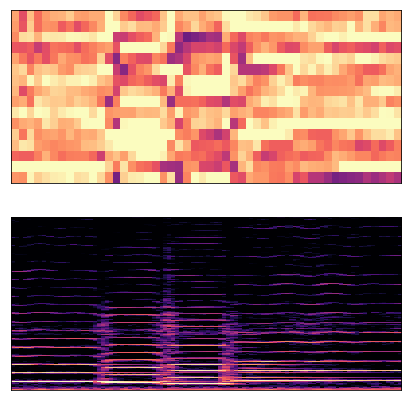
\includegraphics[width=\textwidth]{figures/time_distributed_z_baseline.png}
        \small Baseline
    \end{minipage}
    \hfill
    \begin{minipage}[b]{0.3\textwidth}
        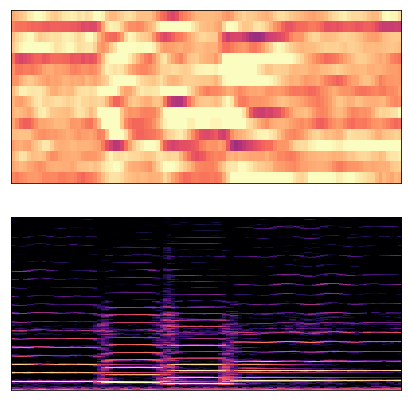
\includegraphics[width=\textwidth]{figures/time_average_z_baseline.png}
        \small Time-averaged z model
    \end{minipage}
    \hfill
    \begin{minipage}[b]{0.3\textwidth}
        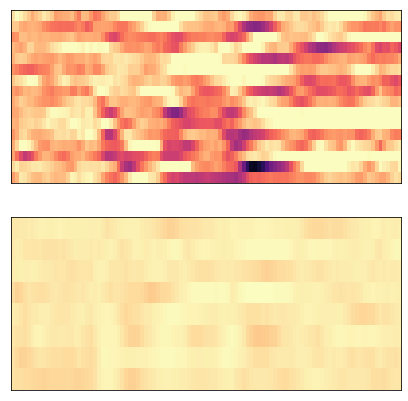
\includegraphics[width=\textwidth]{figures/time_groupwise_z_improved.png}
        \small Confidence-masked z model
    \end{minipage}
    \caption{The latent variable $z$ varies over time} 
    \small In the top row, the decoder output for $z$ is displayed. The baseline model (left) passes $z$ as a time distributed variable to the decoder, which only learns to synthesize natural audio for melodies if the corresponding $z$ is presented, leading to poor timbre transfer performance.
    The time-averaged $z$ model (middle) uses the mean of all $z$ values as the input to the decoder, which leads to a much better timbre transfer performance as the decoder learns to deal with noisy $z$ inputs, which can be obtained from a single recording of the target instrument.
    The confidence-masked $z$ model (right) predicts a confidence mask (bottom row) for each $z$ value and computes a weighted mean. This enables the model to infer certain dimensions of $z$ from different parts of the audio.
    \label{fig:baseline-z-t}
\end{figure}

Surprisingly, it is still possible for a time-constant $z$ model to achieve a comparable reconstruction error as the baseline by introducing a few additional tweaks. One of them directly addresses the problem of noisy $z$ estimates. During a recording, there may be silent parts that should not be taken into account when computing $z$, and different parts of the audio signal can contain different information about the timbre. \newline
So rather than simply averaging along the time axis, the confidence-masked $z$ model predicts a confidence mask for each $\hat{z}$ value and computes a weighted mean.
\begin{equation}
    \begin{split}
        x &= \alpha_{enc}(A) \\
        \hat{c} &= sigmoid(\alpha_c(x)) \\
        c &= \hat{c} / \sum_t \hat{c}_t \\
        \hat{z} &= \alpha_z(x) \\
        z &= \sum_t (\hat{z} * c)_t
    \end{split}
\end{equation}
Here, $\alpha_{enc}$ is a neural network with the same architecture as the baseline encoder, and $\alpha_c$ and $\alpha_z$ are time distributed linear layers.
This enables the model to infer certain dimensions of $z$ from different parts of the audio.
The additional changes explained in the following sections were also used for the confidence-masked model.


\renewcommand{\arraystretch}{0.8}
\begin{figure}
    \centering
    \begin{tabular}{l|c c c}
        & Baseline & Time-averaged z model & Confidence masked z model \\
        \hline
        \rotatebox[origin=c]{90}{Reconstruction} &
        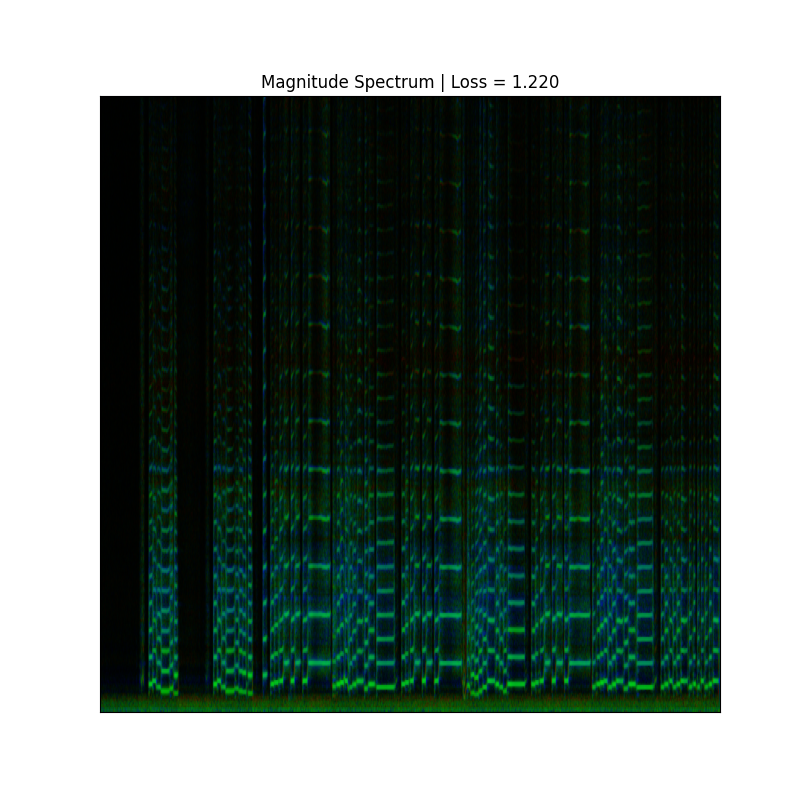
\includegraphics[valign=m,width=140px]{figures/heatmaps/reconstruction_baseline.png} &
        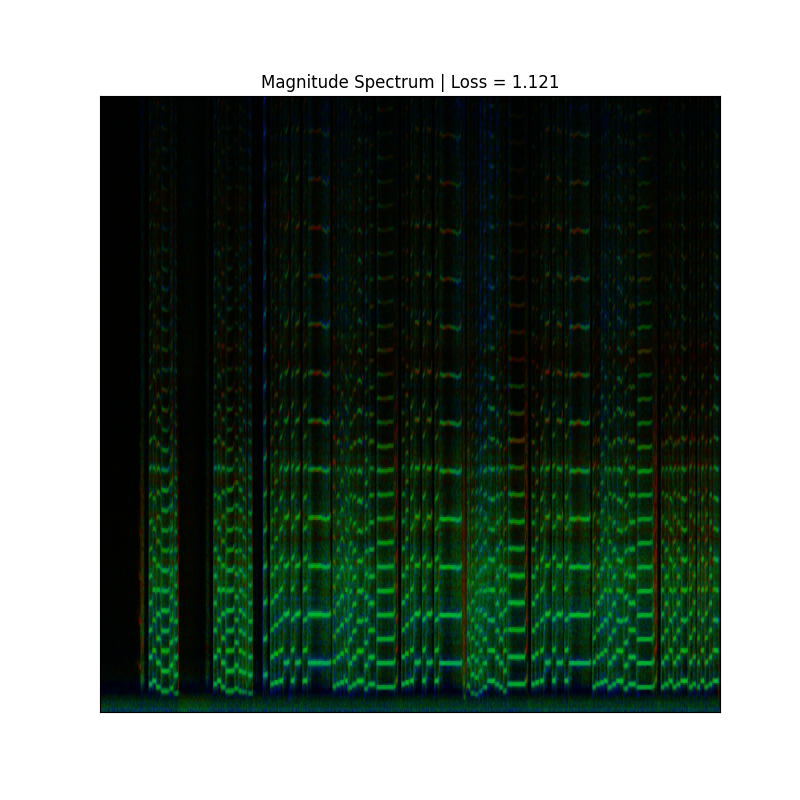
\includegraphics[valign=m,width=140px]{figures/heatmaps/reconstruction_average.png} &
        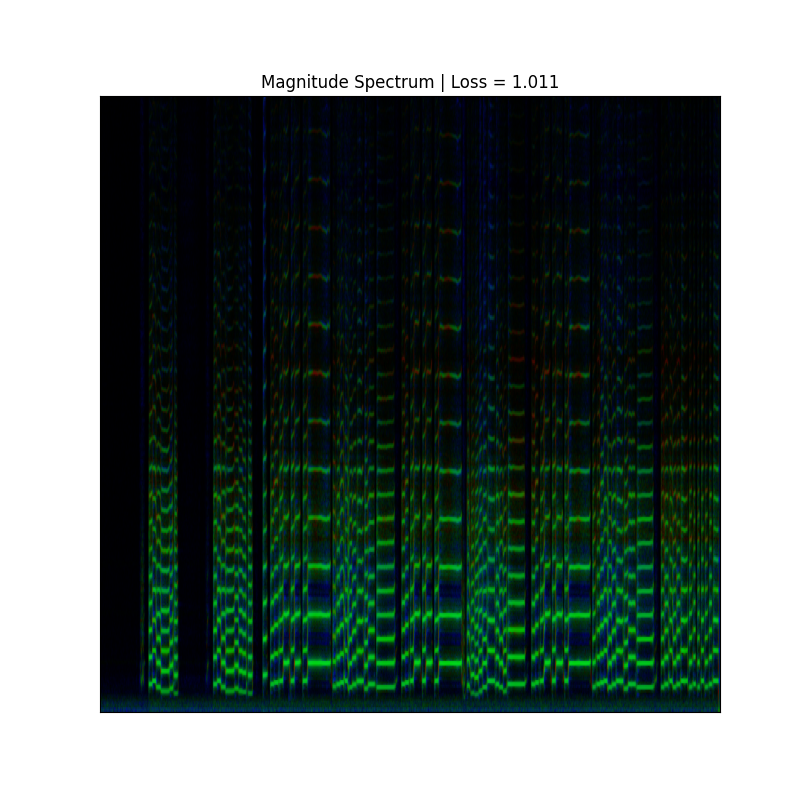
\includegraphics[valign=m,width=140px]{figures/heatmaps/reconstruction_improved.png} \\
        \rotatebox[origin=c]{90}{Cycle Reconstruction} &
        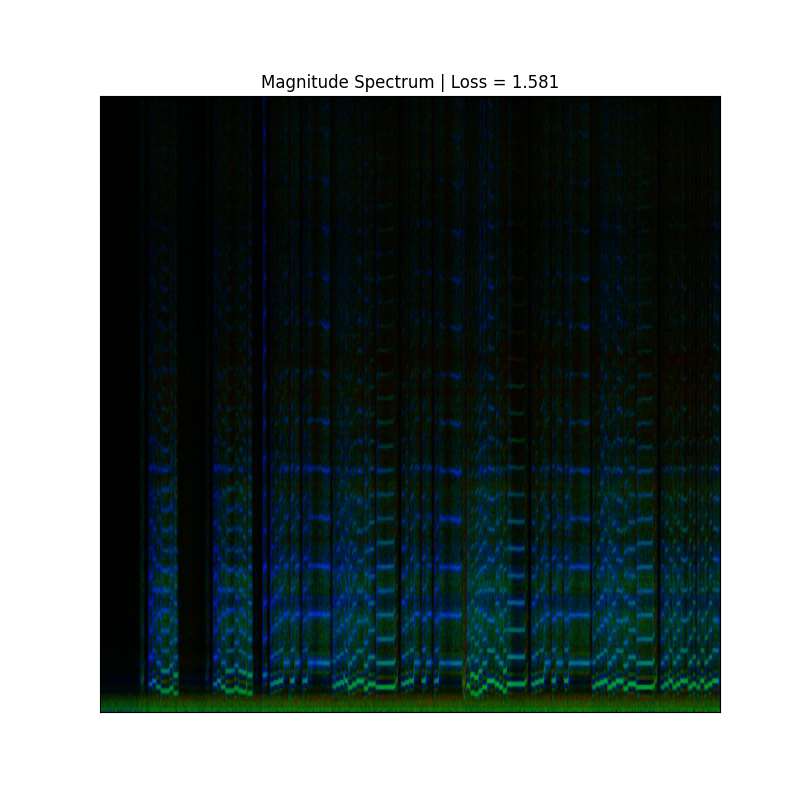
\includegraphics[valign=m,width=140px]{figures/heatmaps/cycle_baseline.png} &
        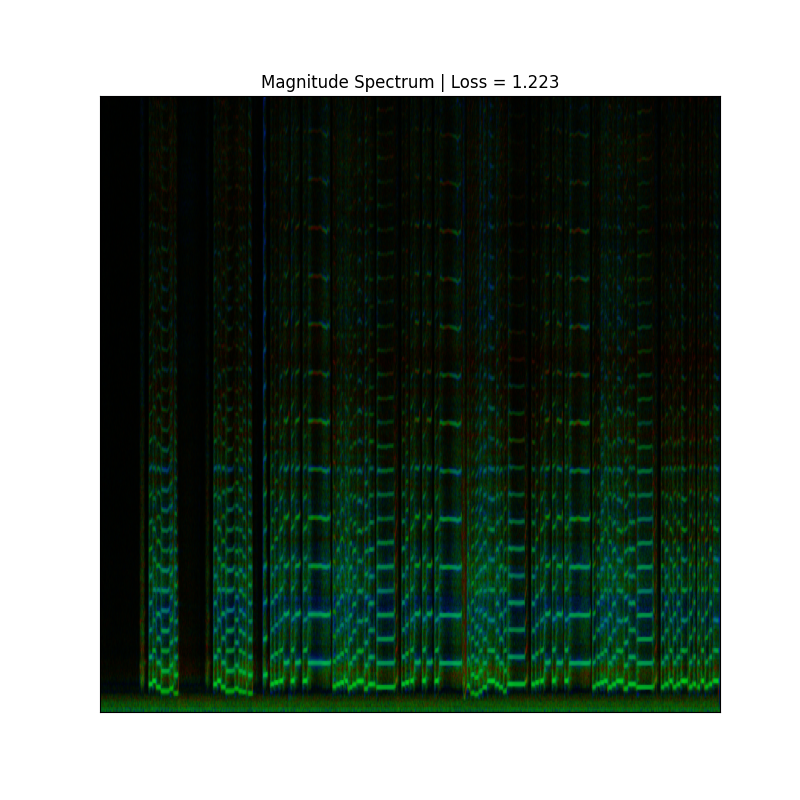
\includegraphics[valign=m,width=140px]{figures/heatmaps/cycle_average.png} &
        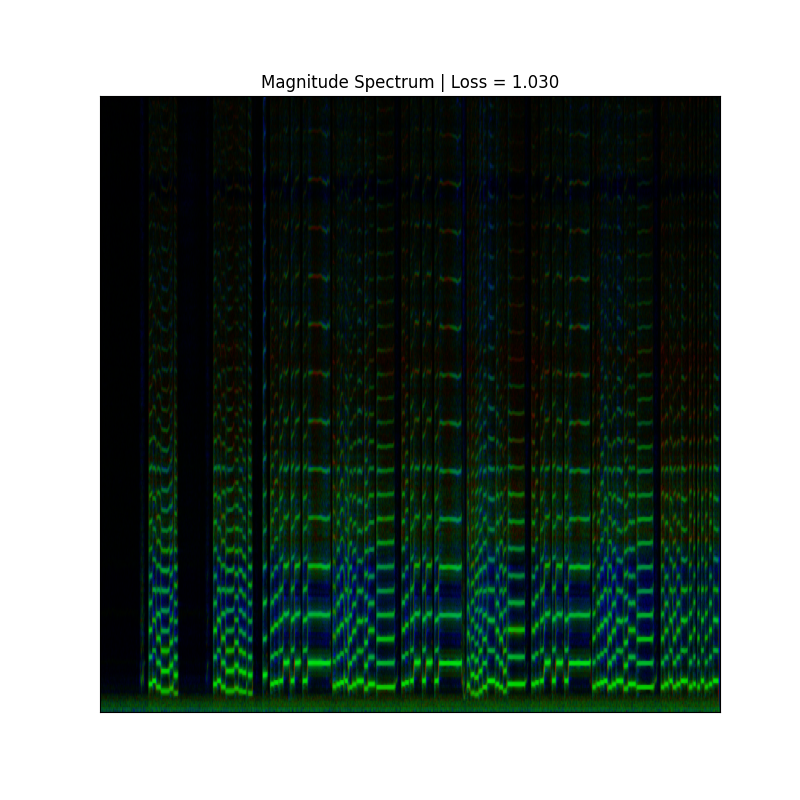
\includegraphics[valign=m,width=140px]{figures/heatmaps/cycle_improved.png} \\
    \end{tabular}
    \caption{A time-constant $z$ model outperforms the baseline in terms of cycle reconstruction loss} 
    \label{fig:cycle-reconstruction-error-exp1}
    \small These error heatmaps visualize the difference between the spectrogram of some original audio and its reconstructed version. Frequencies present in both the original and the synthesized audio are shown in green, red shows where the synthesized audio is too loud and blue highlights, where the synthesized audio is missing frequencies.
\end{figure}


\subsection{Loudness}

In psychoacoustics, loudness describes the perceived intensity of a sound.
Unlike the spectral power or amplitude, loudness is not defined in a precise mathematical way.
There are algorithms for approximating loudness that are used in the DDSP autoencoder.
To compute loudness, a power spectrum is computed and converted into a decibel scale.
In order to take into account that for most people the loudness of a sound depends not only the power but also on the frequency at which it appears, A-weighting is applied. A-weighting scales the activations of the power spectrogram by a constant factor depending on the frequency.
The weighted power spectrum is then meaned along the frequency axis to obtain the loudness curve.
A visualization of this process is displayed in \Cref{fig:loudness}. \newline
The official DDSP implementation uses A-weighting by adding a per-frequency bias to the power decibel spectrogam. The resulting spectrogram is then averaged over the frequency axis, such that the A-weighting becomes ineffective: it only shifts the complete loudness curve by its mean value.  \newline
The oscillation of the loudness curve that can be seen in \Cref{fig:loudness} are due to another issue.
During the signal, the frequency of the loudness varies, but the spectrogram only has a discrete number of frequency bins.
Whenever the instantaneous frequency is not close to the center of a frequency bin, the spectrogram gets a bit blurred along the frequency axis. This phenomenon is called spectral leakage.
If we now transform the power spectrum into the decibel scale, we apply a concave function. As is known from Jensen's inequality, the mean of these values will be much larger than if all the power at the timestep would fall into a single frequency bin. Therefore, loudness oscillates as the instantaneous frequency moves between frequency bins. \newline
% new loudness applies a-weighting in as multiplication in the linear power spectrum - equivalent to adding in the log scale
To fix these bugs, I computed loudness by applying a-weighting as a multiplication in the power spectrum, which is equivalent to adding a bias in the log-scale.
Then, I applied a mean over the frequency axis to obtain the loudness curve and applied the logarithm as the last step. A detailed discussion of this algorithm can also be found in the corresponding github issue \footnote{\href{https://github.com/magenta/ddsp/issues/361}{github.com/magenta/ddsp/issues/361}}.
A model trained with the adjusted loudness algorithm improves particularly in silent parts, where the model otherwise puts an unpleasant squeaky noise as it does not have reliable information on the true loudness. Such an example is shown in \Cref{fig:loudness-rec}.
% then means along the frequency axis and converts to dB in the last step
% before taking the mean, values below a threshold


\begin{figure}
    \centering
    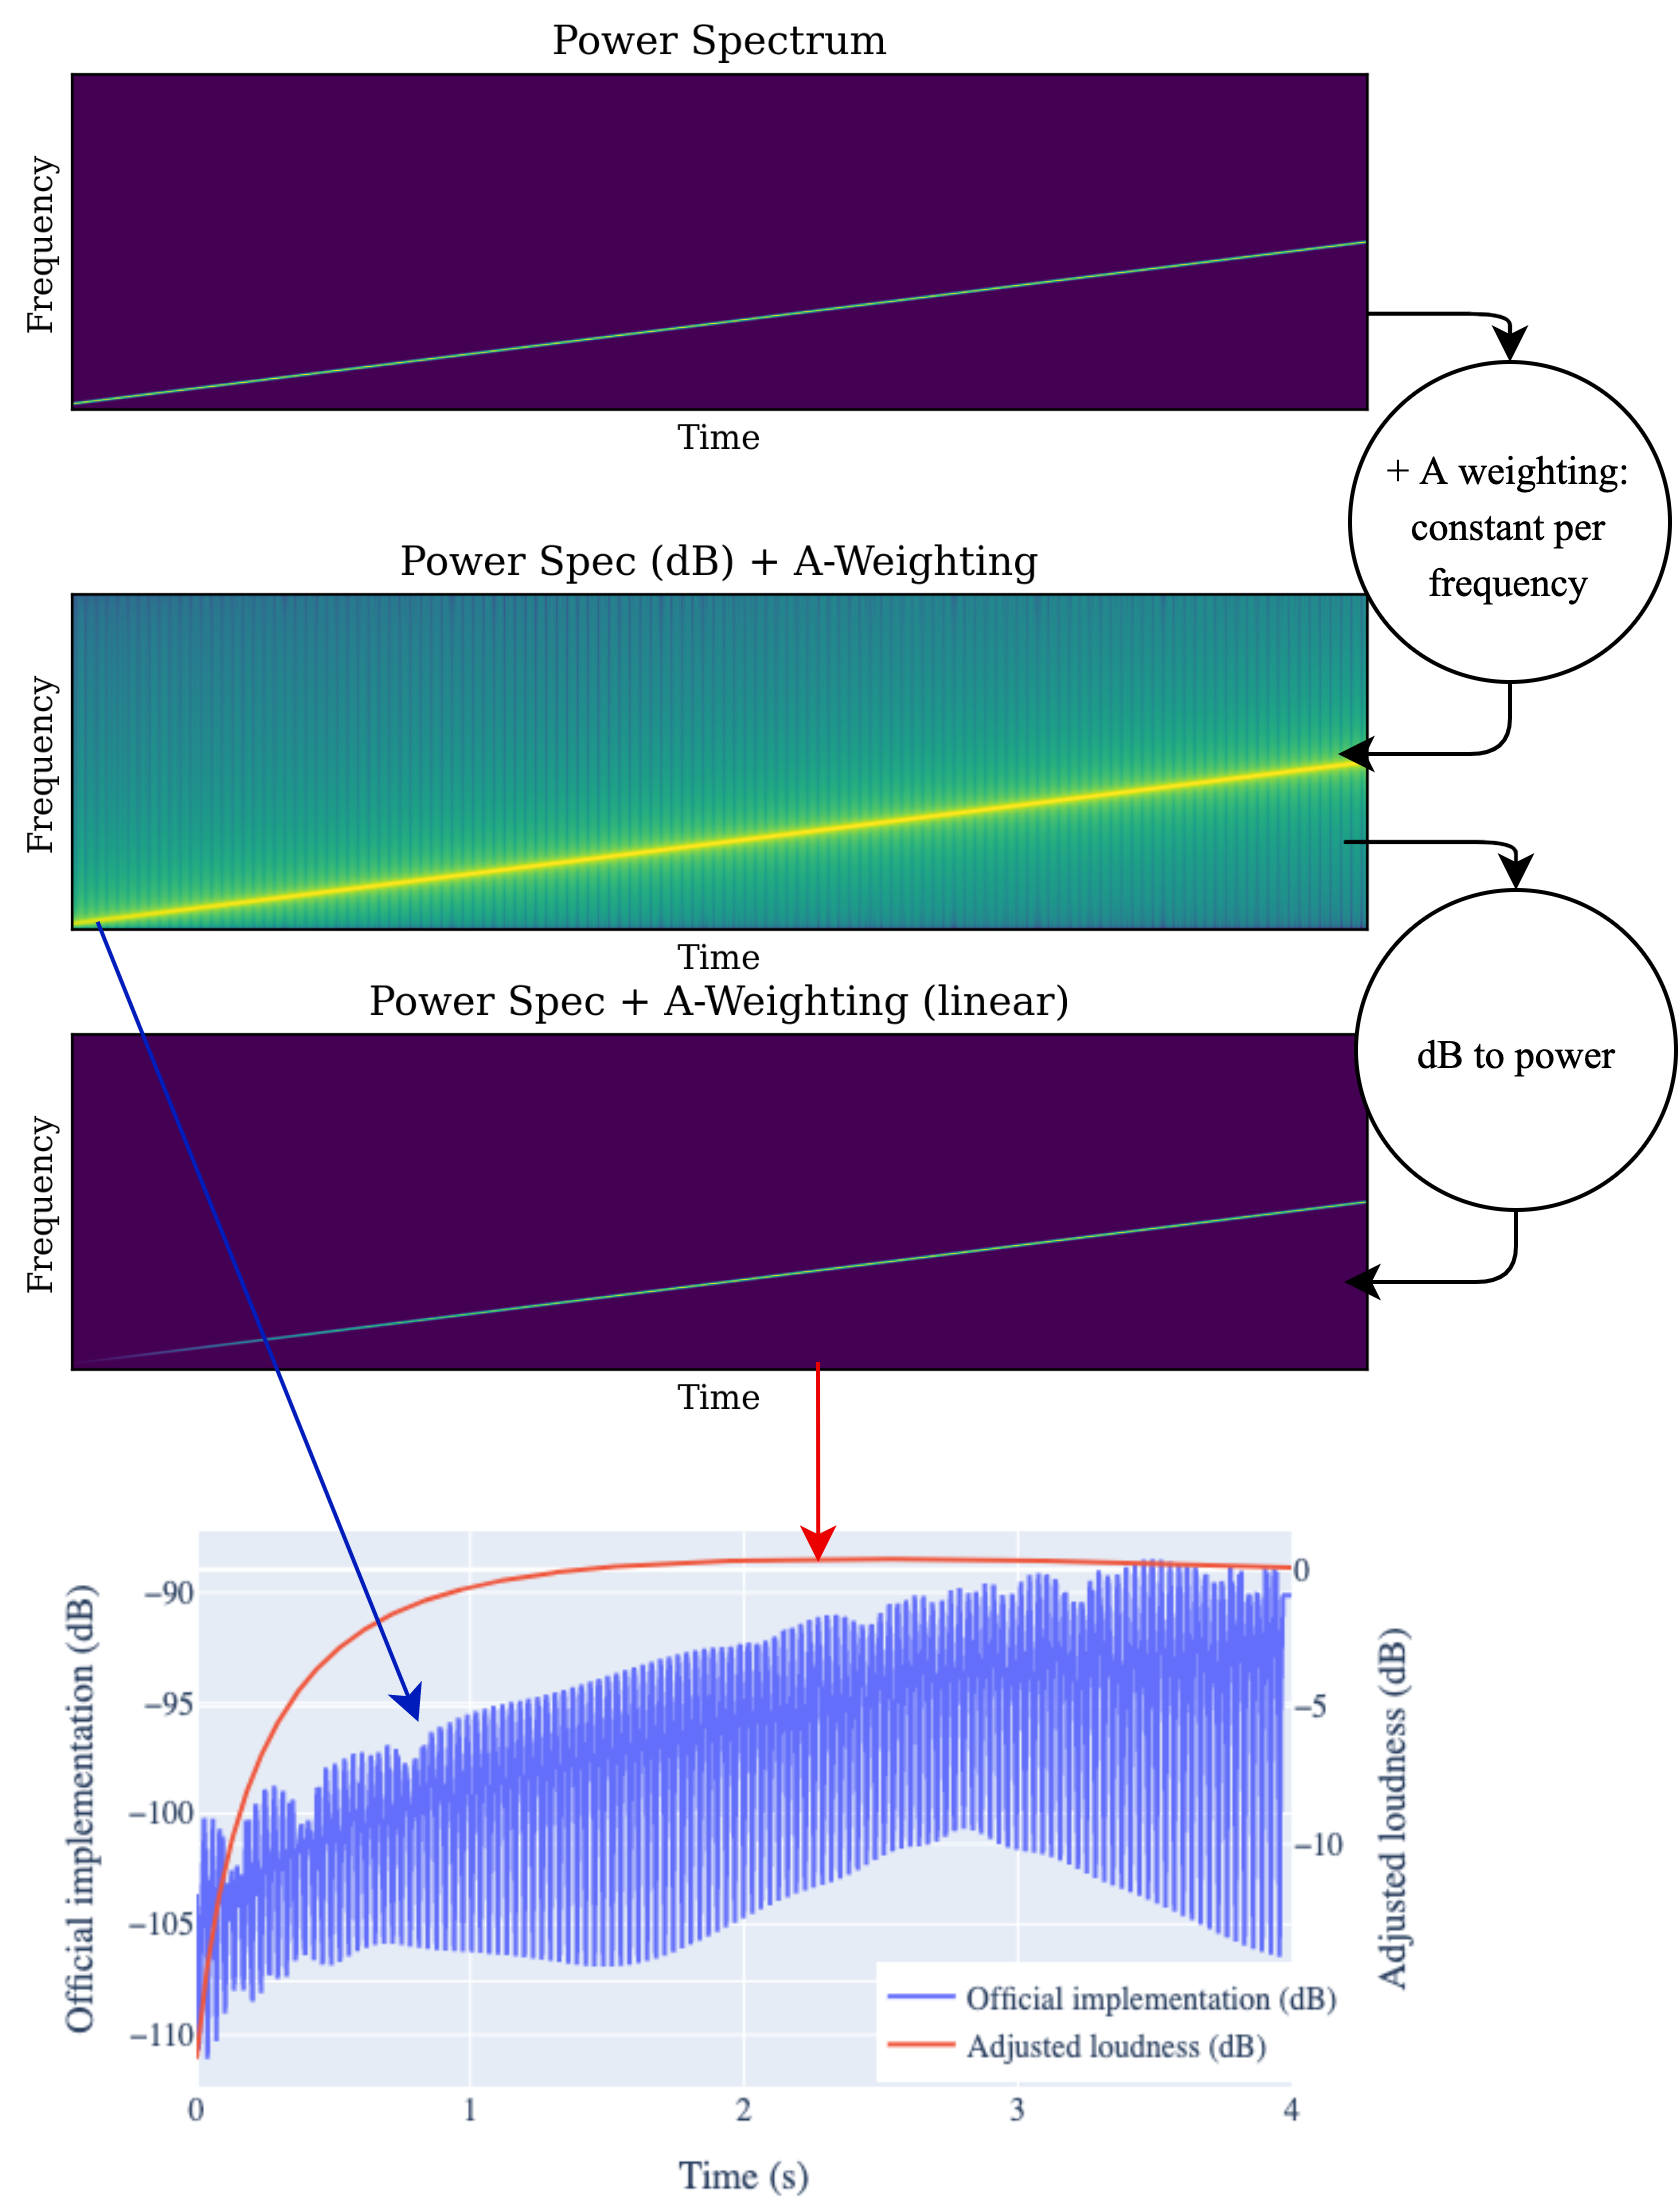
\includegraphics[width=350px]{schema/loudness.png}
    \caption{Computing loudness}
    \small Two loudness curves for the same audio signal are shown here: the signal is a single sine wave with a frequency starting at 100Hz and going to 4000Hz. A bug in the algorithm for computing loudness makes the loudness curve sensitive to artifacts of the spectrogram. The resulting loudness curve for the pitch sweep oscillates strongly as frequency leakage occurs in the spectrogram. The loudness algorithm used for the improved baseline fixes this and produces a smooth loudness curve that is shaped by the A-weighting.
    \label{fig:loudness}
\end{figure}

\begin{figure}
    \centering
    \begin{minipage}[b]{0.45\textwidth}
        \centering
        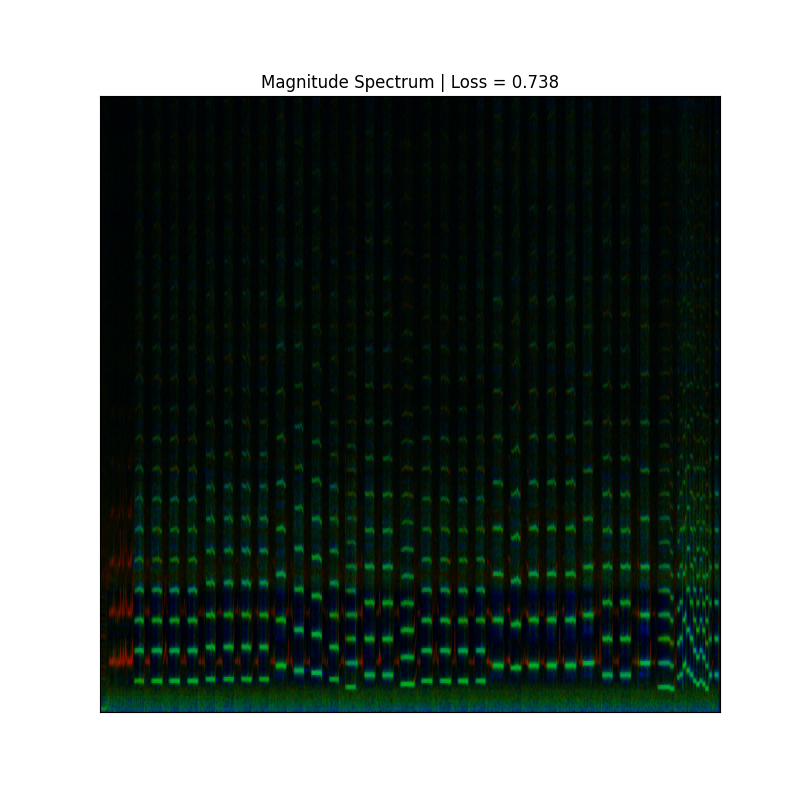
\includegraphics[width=\textwidth]{figures/loudness/reconstruction_baseline.png}
        \small Time average $z$ + old loudness
    \end{minipage}
    \hfill
    \begin{minipage}[b]{0.45\textwidth}
        \centering
        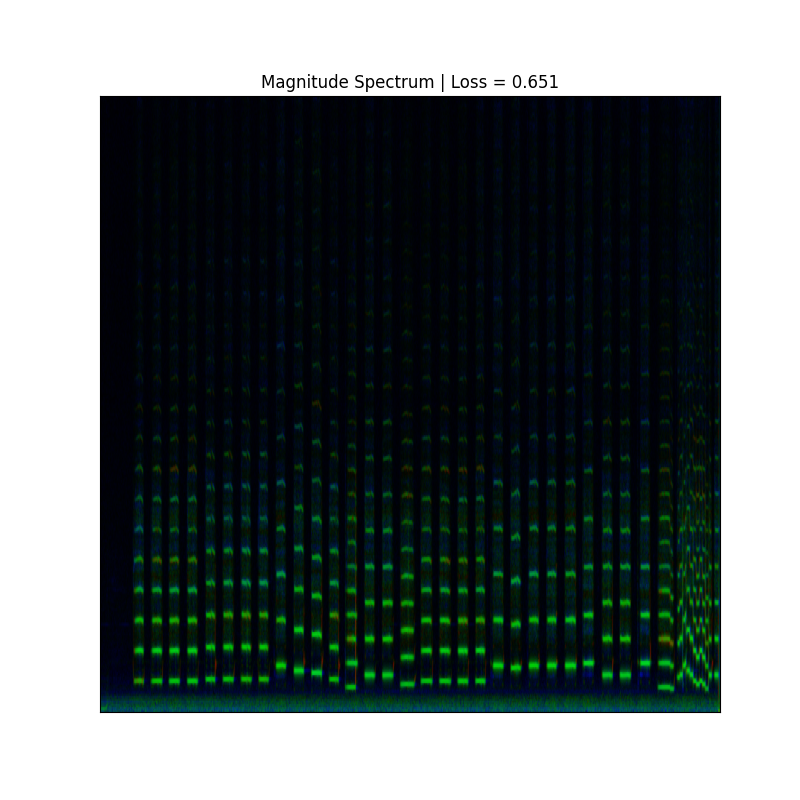
\includegraphics[width=\textwidth]{figures/loudness/reconstruction_new_loudness.png}
        \small Time average $z$ + adjusted loudness
    \end{minipage}
    \caption{A reconstruction using the official vs the adjusted loudness algorithm}
    \label{fig:loudness-rec}
    \small Two models reconstruct a 30 second audio recording of a flute playing. The models only differ in the loudness algorithm used, all other parameters are identical. In the reconstruction using the old loudness (left) the model creates an unpleasant squeaky noise in the silent beginning of the audio. A model trained with the adjusted loudness algorithm (right) does not have this problem.
\end{figure}

\subsection{Multi-Scale Spectrogram Loss}
Two very different waveforms can sound the same, for example, if they are overlayed sine waves with the same frequencies in different phases.
Therefore, it is problematic to use a mean-squared error loss function of the waveform in order to evaluate a reconstruction.
Some models like WaveNet follow this approach, but the task is more complex than it needs to be: instead, the difference between the two spectrograms can be used to compute the loss.  \newline
A common approach to do so is via a multi-scale spectrogram (MSS) loss.
Since the phase information is lost in the spectrogram, the MSS loss is invariant to phase shifts, like the human perception. 
For the MSS loss, multiple spectrograms of the audios are computed with different window sizes.
A spectrogram with a large window size has a high frequency resolution but a low temporal resolution, whereas a spectrogram with a small window size has a low frequency resolution but a high temporal resolution.
The MSS loss is then computed by summing the absolute difference between the two spectrograms. It therefore has a high resolution in both frequency and temporal dimensions. \newline
\cite{ddsp} and other work use magnitude spectrograms and log-magnitude spectrograms with window sizes ranging from 4ms to 128ms.
These spectrograms are shown in \Cref{fig:mss-loss}. \newline
Ideally, the spectrogram magnitudes are scaled such that the resulting loss function aligns with the human perception.
A good indicator for this is if audible mistakes are also visible in the spectrogram difference.
When playing around with visualizing the difference between two audios, I found the scaling of the baseline implementation not to be ideal.

The logmag-spectrograms look noisy, but the amplitude spectrograms have such a skewed distribution that many perceptually relevant features are hardly visible. As a solution, I unskewed the activation distribution of the magnitude spectrogram with the function
\begin{equation}
    \label{eq:unskew}
u(M, s) = log(1 + s * M)
\end{equation}
where $M$ is the magnitude spectrogram, and $s$ is a scalar smoothing factor.
High values for $s$ also highlight differences in low-energy parts of the spectrogram but are less sensitive to differences in parts of the spectrogram that are loud and contain high energy. Example spectrograms with different smoothing factors are shown in \Cref{fig:mss-loss}.
\begin{figure}
    \centering
    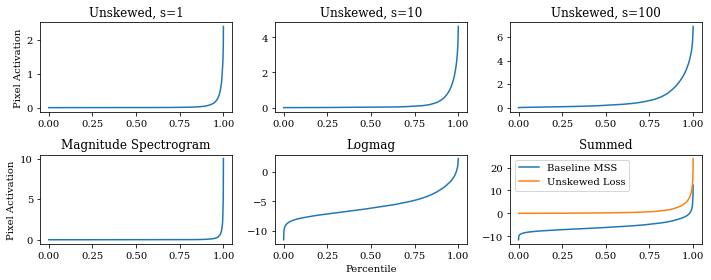
\includegraphics[width=\textwidth]{figures/mss/unskewing.png}
    \caption{Pixel activation distribution of differently scaled spectrograms}
    \small{Looking at the distribution of activations in the spectrograms, it can be seen that the magnitude spectrograms have a highly skewed distribution: only a few pixels are activated a lot, and most pixels have a very low activation. Unskewing with a smoothing parameter $s$ as described in \Cref{eq:unskew} therefore makes patterns in the spectrogram visible that have comparably small activations. The logmag-spectrogram also achieves this, but it is also sensitive to differences in the least activated pixels, which correspond to very quiet frequencies that are likely not audible to most humans.}
    \label{fig:smoothing}
\end{figure}

If we evaluate all trained models for this thesis \footnote{A full list is given in \Cref{table:trainingdetails}}, we observe as expected that the two loss functions produce correlated scores, see \Cref{fig:unskewed-vs-spectral}.
However, models also tend to perform comparably better on the loss function they have been trained to optimize.
A fair comparison of models trained with different loss functions is therefore difficult.
Whether or not the unskewed loss really reflects human perception better is not entirely clear and would require confirmation by multiple human listeners. For the evaluations in this thesis, the unskewed loss was chosen as the default metric.

\begin{figure}
    \centering
    \includegraphics[width=\textwidth]{figures/mss/spectral_diff.png}
    \caption{Spectrograms used to compute the MSS loss}
    \small{The baseline MSS uses only the magnitude and log-magnitude spectrograms (first and last row). The unskewed loss uses the magnitude spectrums with different smoothing factors $s$. These spectrograms visually highlight more differences that can also be heard.}
    \label{fig:mss-loss}
\end{figure}


\begin{figure}
    \centering
    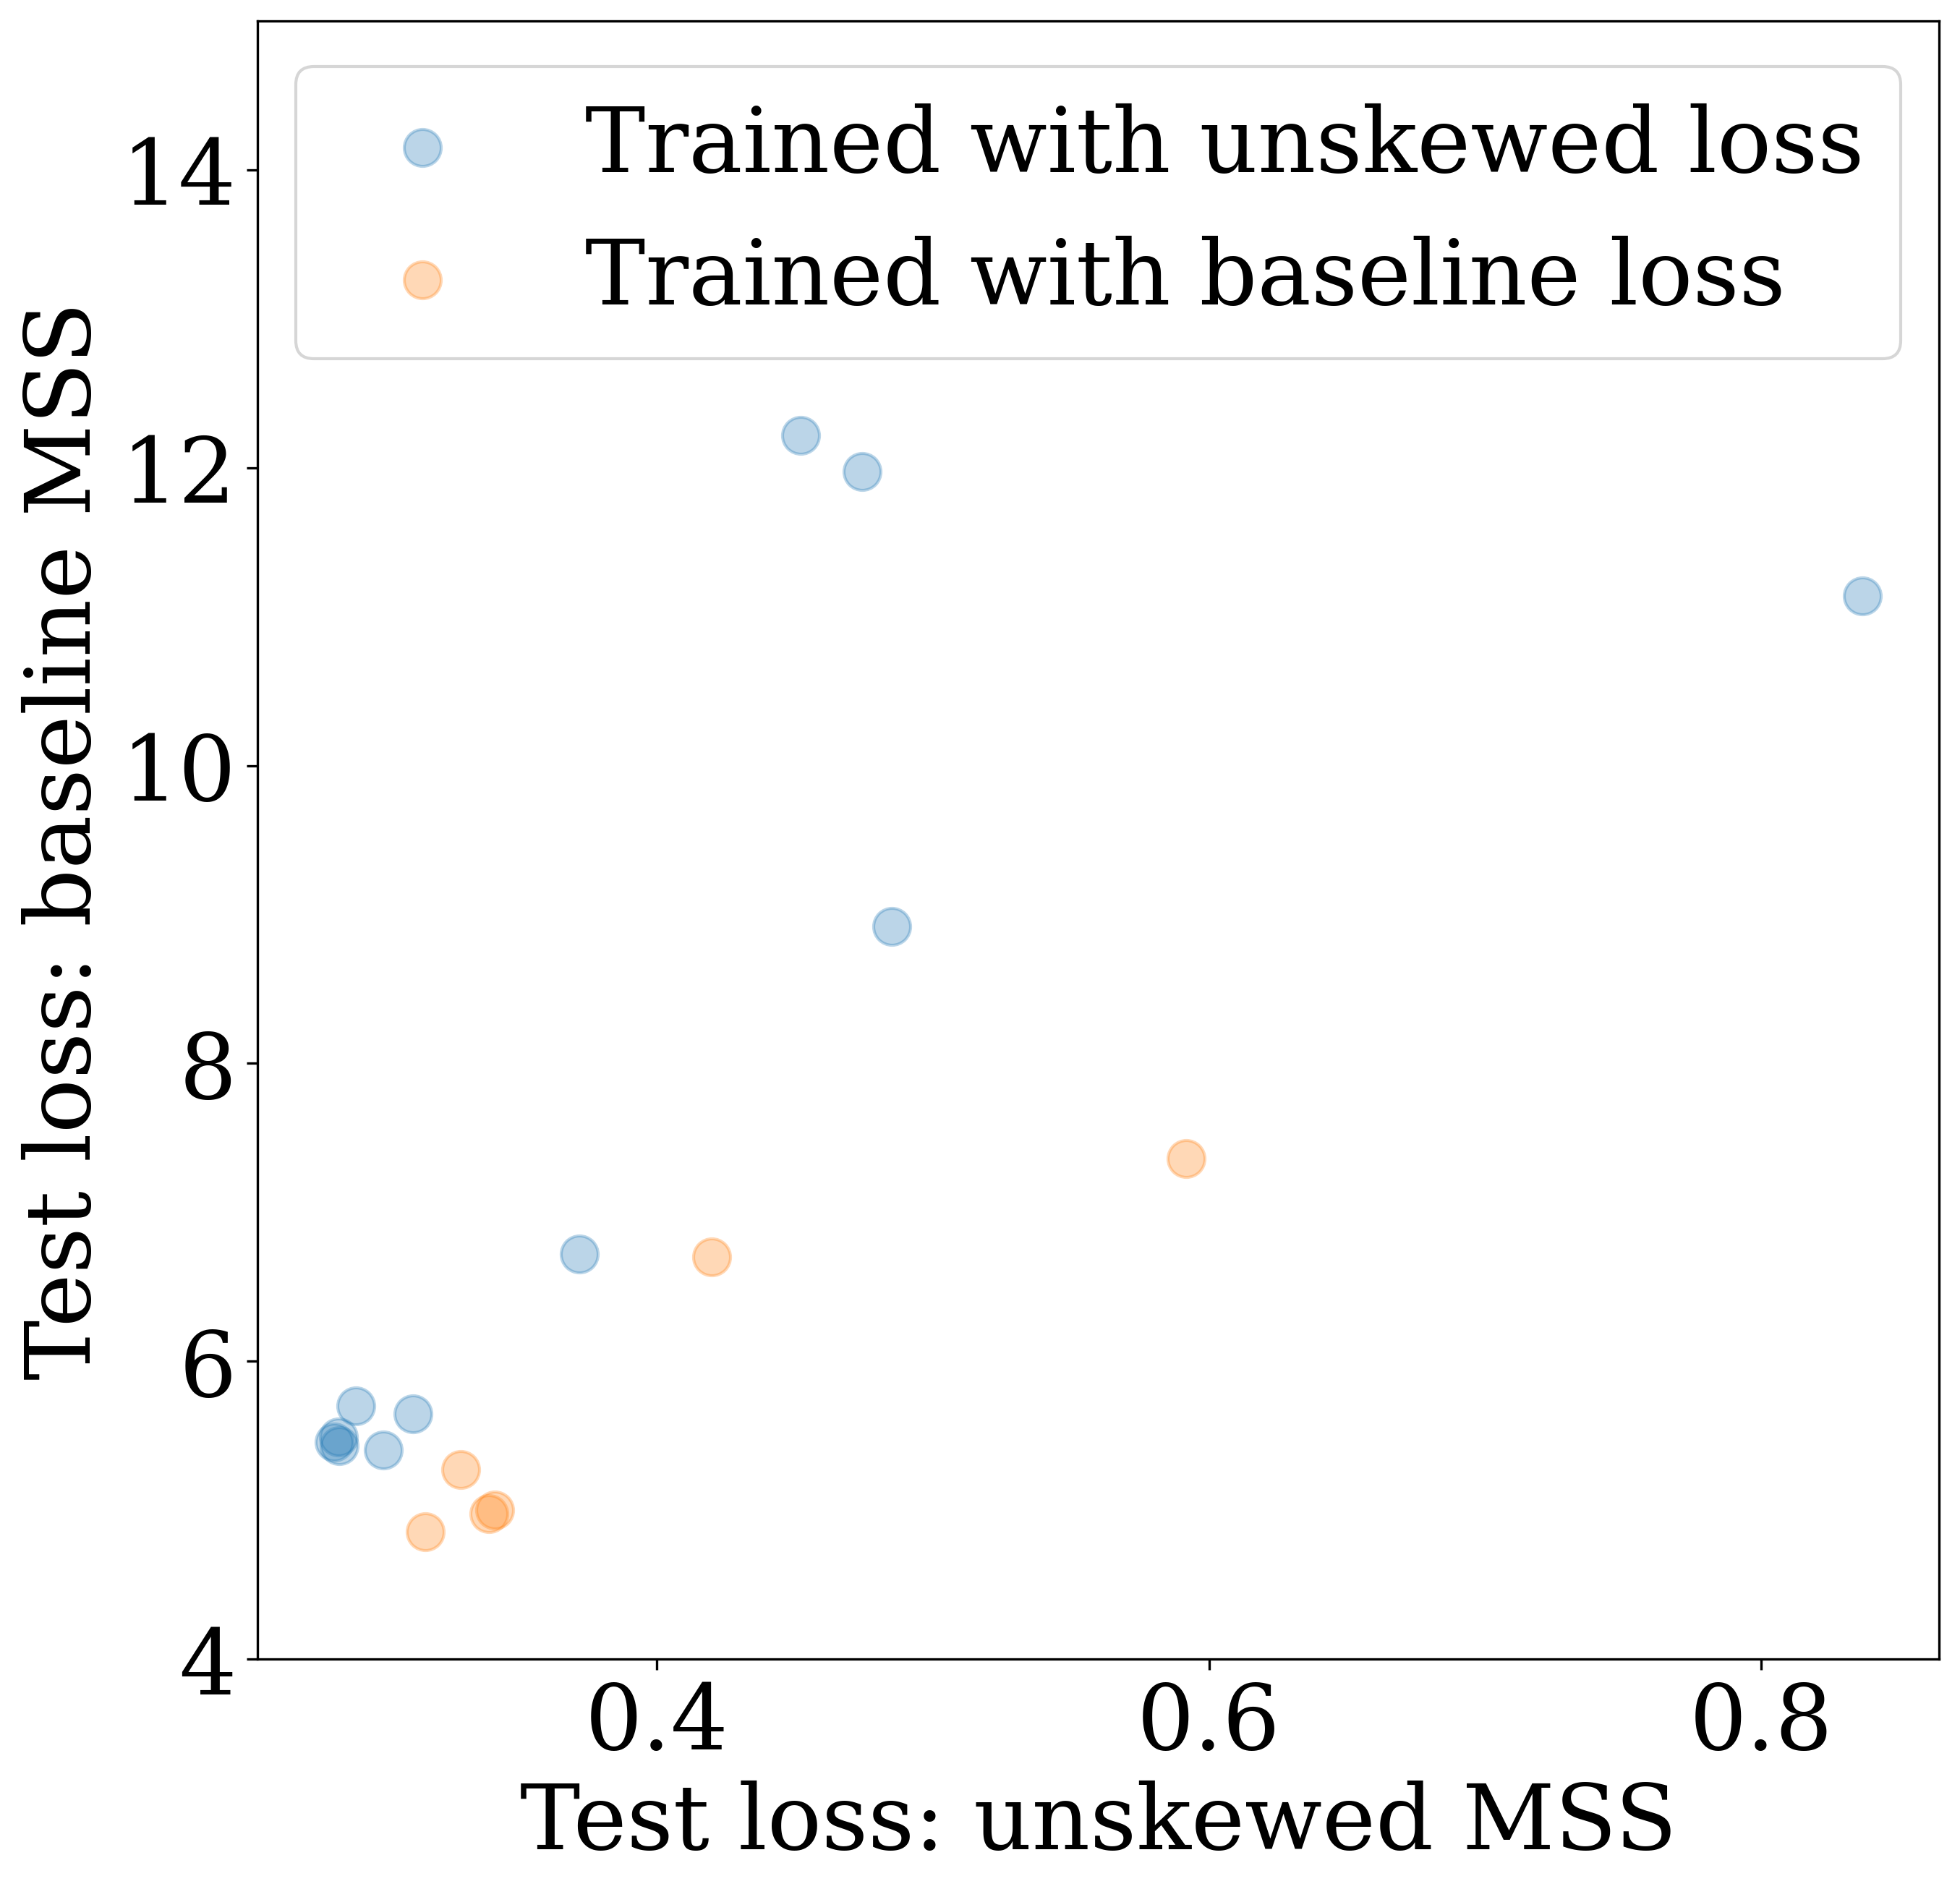
\includegraphics[width=0.5\textwidth]{figures/mss/performance_scatter.png}
    \caption{Test loss evaluated with unskewed MSS vs baseline MSS}
    \label{fig:unskewed-vs-spectral}
\end{figure}


% Grammarly ab hier

\subsection{Bringing it all together}
\label{ablations-summary}
To validate the ideas proposed in the previous sections, I trained a number of models with different configurations. They differ in how they aggregate $z$, which loss function they optimize, and how they compute loudness. These models were then evaluated on all test datasets separately to compute the reconstruction loss. Additionally, on a subset of this test set timbre transfer has been evaluated using the cycle-reconstruction loss. As intermediate melodies, a sample of a guitar playing and a person singing are used. A summary of the results for the URMP test set is shown in \Cref{fig:ablations}. The reason to use only a subset of the test set for evaluating the cycle reconstruction loss lies in the amount of data produced: the total size of produced artifacts at the time of writing this is 14.7GB already. \newline
It can be seen that aggregating $z$ via a mean over the time axis improves timbre transfer but hurts reconstruction.
However, using the u-MSS and the adjusted loudness algorithm improve the performance such that the improved baseline beats the baseline in both timbre transfer and reconstruction. 
The architectural design composed of the best individual choices is therefore the one that
\begin{itemize}
    \item Uses confidence-masked $z$-aggregation in the encoder,
    \item is trained with the unskewed MSS loss and
    \item uses the fixed loudness algorithm.
\end{itemize}
Models using all these settings are now referred to as improved baseline models.
\begin{figure}
    \centering
    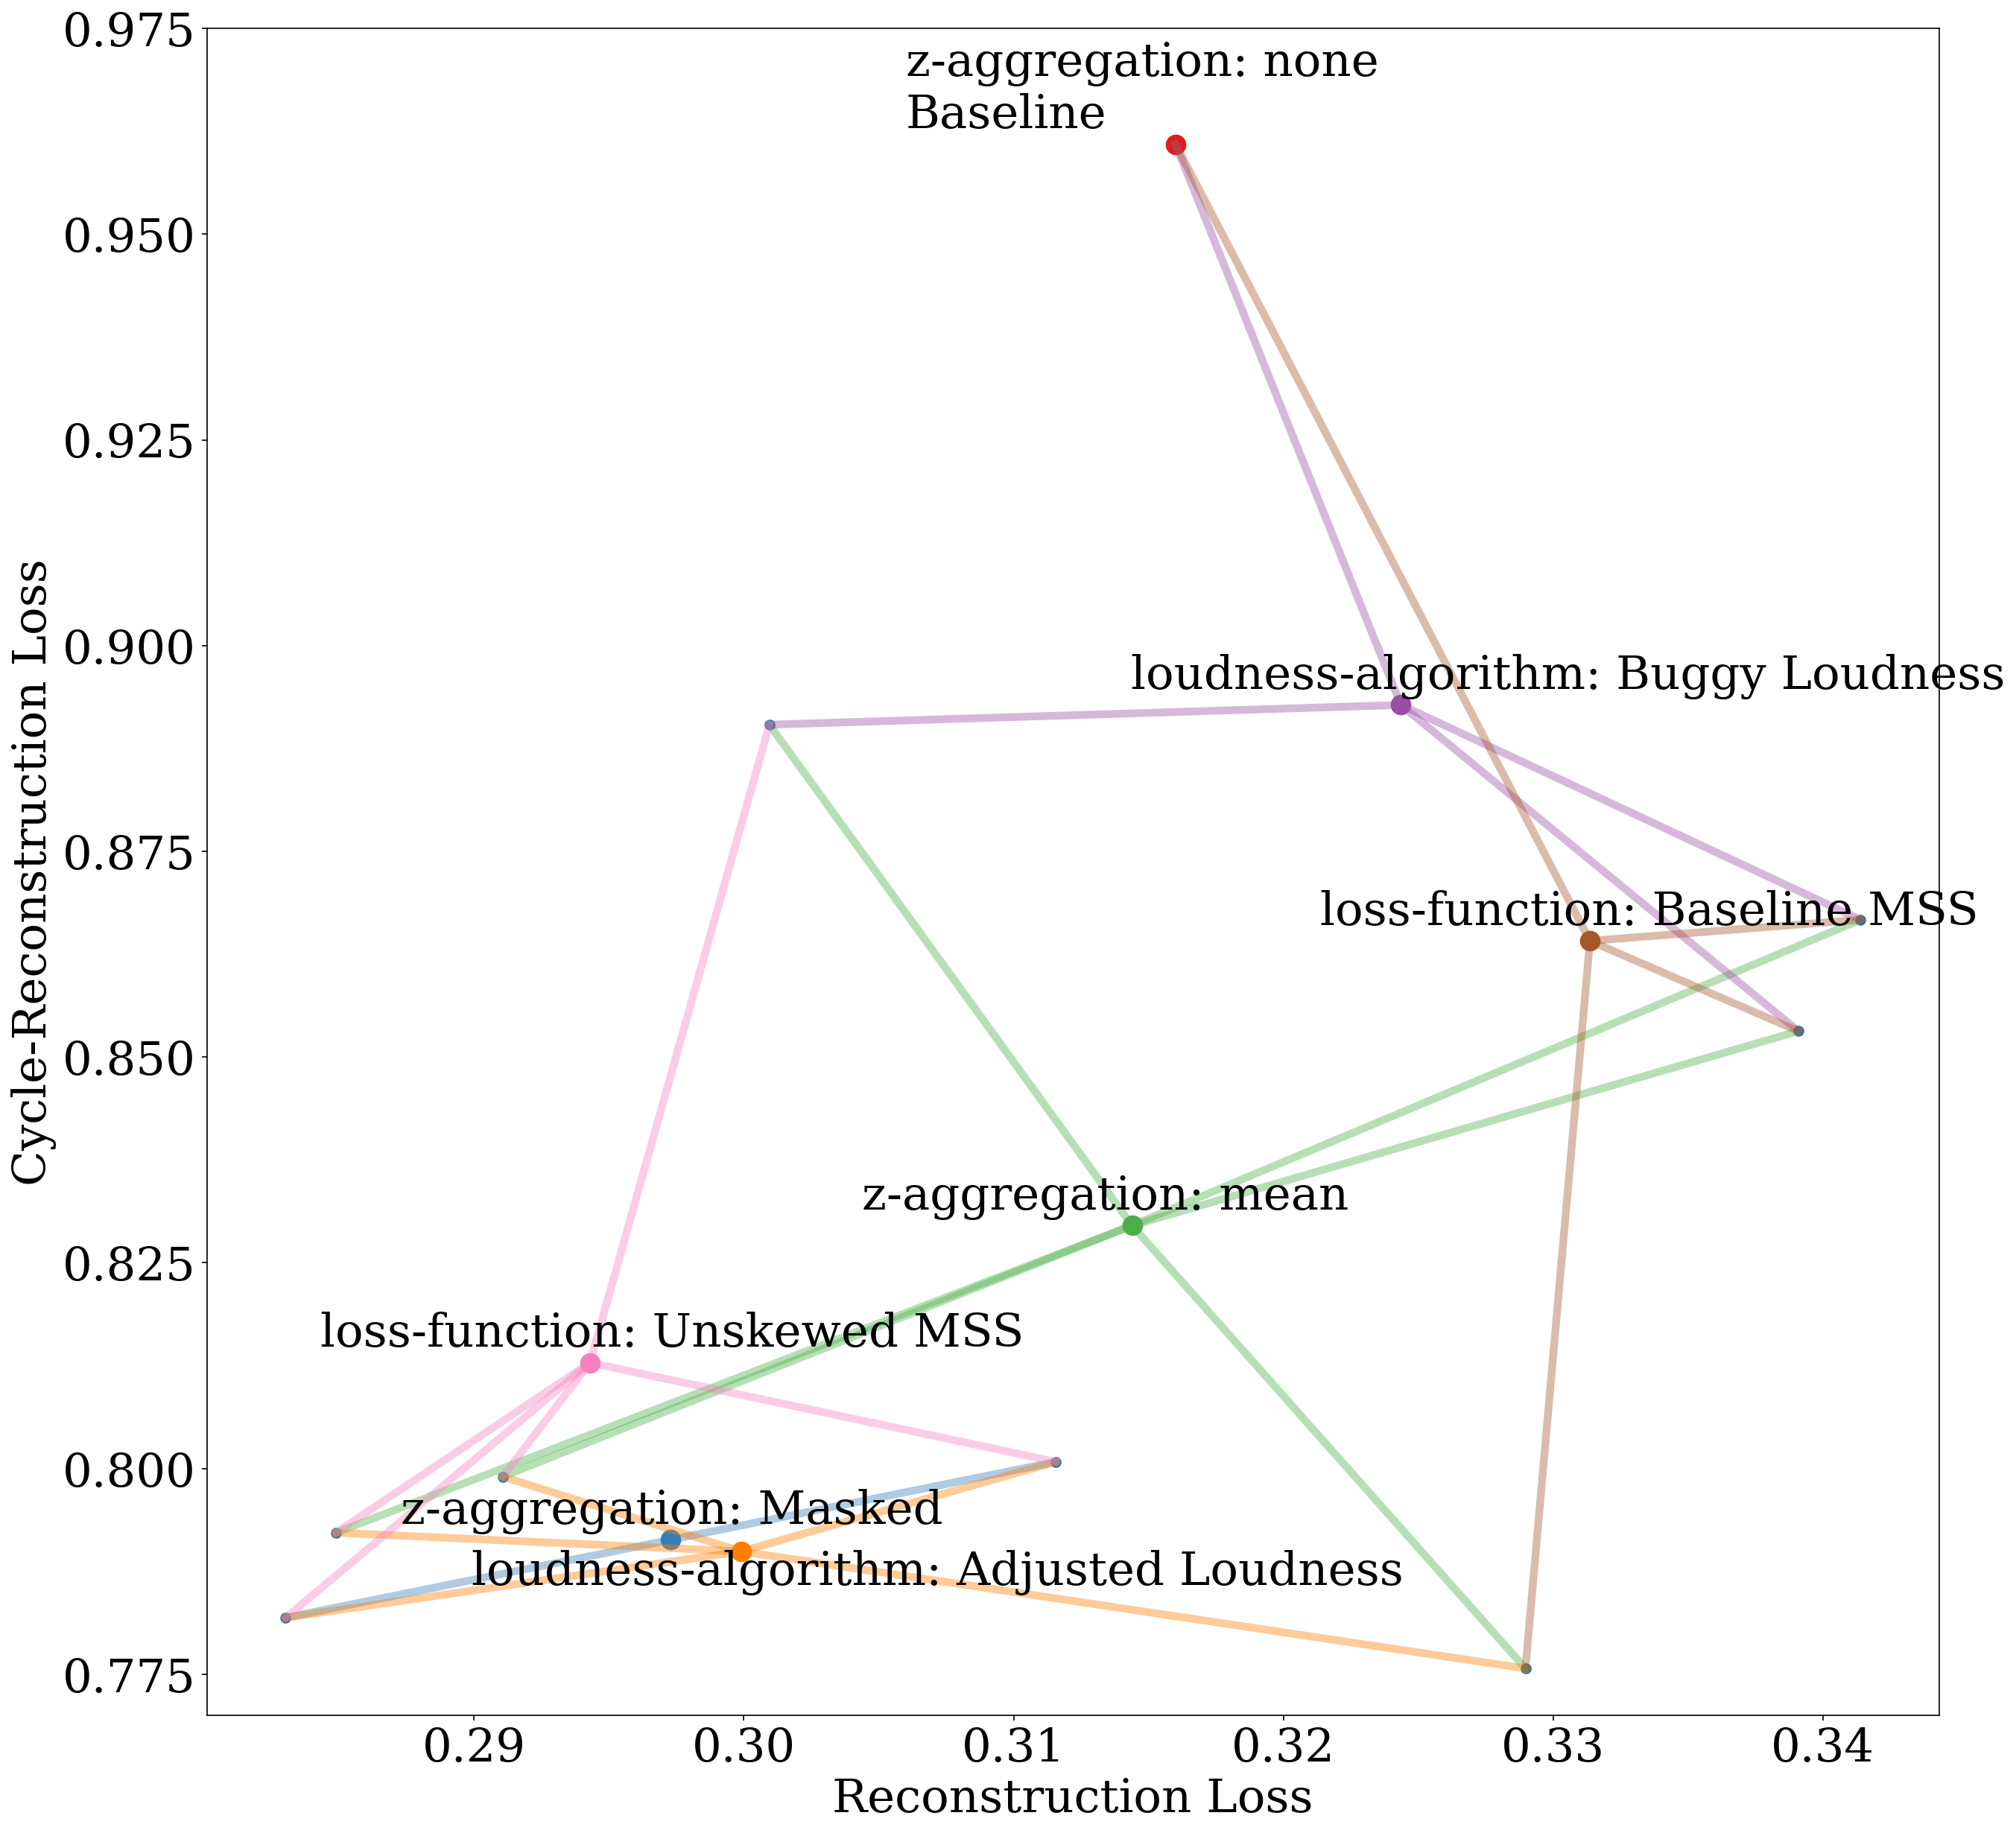
\includegraphics[width=\textwidth]{figures/ablations.png}
    \caption{Comparison of Test Losses on URMP}
    \label{fig:ablations}
    \small{This figure summarizes all metrics of the ablation studies shown in \Cref{tab:ablations-urmp}. Each small blue point corresponds to one model trained on the URMP train dataset. The colored points correspond to the mean performance of all models trained with a certain configuration. Models and configurations are connected to if the model uses this configuration. The baseline model uses the configrations in the upper right, showing that all proposed changes improve the model's reconstruction and timbre transfer performance as measured by cycle reconstruction error.}
\end{figure}

\begin{table}
    \begin{tabular}{lll}
        \multicolumn{3}{c}{Baseline loss, baseline loudness} \\
        \\
        \textbf{z-aggregation} & Reconstrunction u-MSS & Cycle-Reconstruction u-MSS \\
        None  & 0.316* & 0.961 \\
        Mean & 0.341	& 0.867* \\
        \hline
        \\
        \\
        \multicolumn{3}{c}{$z$-aggregation: mean, baseline loudness} \\
        \\
        \textbf{Training objective} & Reconstrunction u-MSS & Cycle-Reconstruction u-MSS \\
        MSS (Baseline) & 0.341 & 0.867* \\
        u-MSS & 0.301* & 0.890 \\
        \hline
        \\
        \\
        \multicolumn{3}{c}{$z$-aggregation: mean, Training objective: u-MSS} \\
        \\
        \textbf{Loudness algorithm} & Reconstrunction u-MSS & Cycle-Reconstruction u-MSS \\
        Loudness (Baseline) & 0.301 & 0.890 \\
        Loudness (fixed) & 0.285* & 0.792* \\
        \hline
        \\
        \\
        \multicolumn{3}{c}{Training objective: u-MSS, Loudness algorithm: fixed} \\
        \\
        \textbf{z-aggregation} & Reconstrunction u-MSS & Cycle-Reconstruction u-MSS \\
        Mean & 0.291 & 0.799 \\
        Confidence-masked & 0.283* & 0.781* \\
        \hline
    \end{tabular}
    \caption{Ablations on URMP}
    \label{tab:ablations-urmp}
\end{table}

The baseline and the improved baseline models have not only been trained and evaluated on the URMP dataset but also all other datasets listed in \Cref{table:datasets}. The improved baseline has additionally been trained on a composition of all other datasets.
This single model compares well on all datasets with a baseline model that has only been trained on the corresponding train set, as \Cref{fig:multi-datasets} shows. Again, it is highly recommended to listen to the examples of the dashboard, as the loss seems to be better for the base model on some data sets like the sh101 data set. However, listening to the examples shows that the timbre transfer and cycle reconstruction of the improved model sound much better than those of the baseline model.
The aim to create a single model that can handle a large number of instruments is thereby partly achieved - yet, the sound quality is not perfect, and the cycle reconstruction loss is consistently much above the reconstruction loss, showing that the models cannot perfectly preserve timbre in a transfer task.
Another finding is that a mixture of experts has slightly better performance than a single model trained on all datasets.
Some of this may be explained by the fact that the mixture of experts trained for five times more steps than the single model and equally has five times more parameters. It might therefore be interesting to train a larger model for more steps on the combined dataset, but this is beyond the scope of this project. \newline
If the dataset consists of a single instrument, the baseline architecture is still a good choice for performing timbre transfer. If the train dataset consists of multiple instruments, as it is the case in the URMP dataset, the improved baseline model is a better choice for timbre transfer.

\begin{figure}
    \centering
    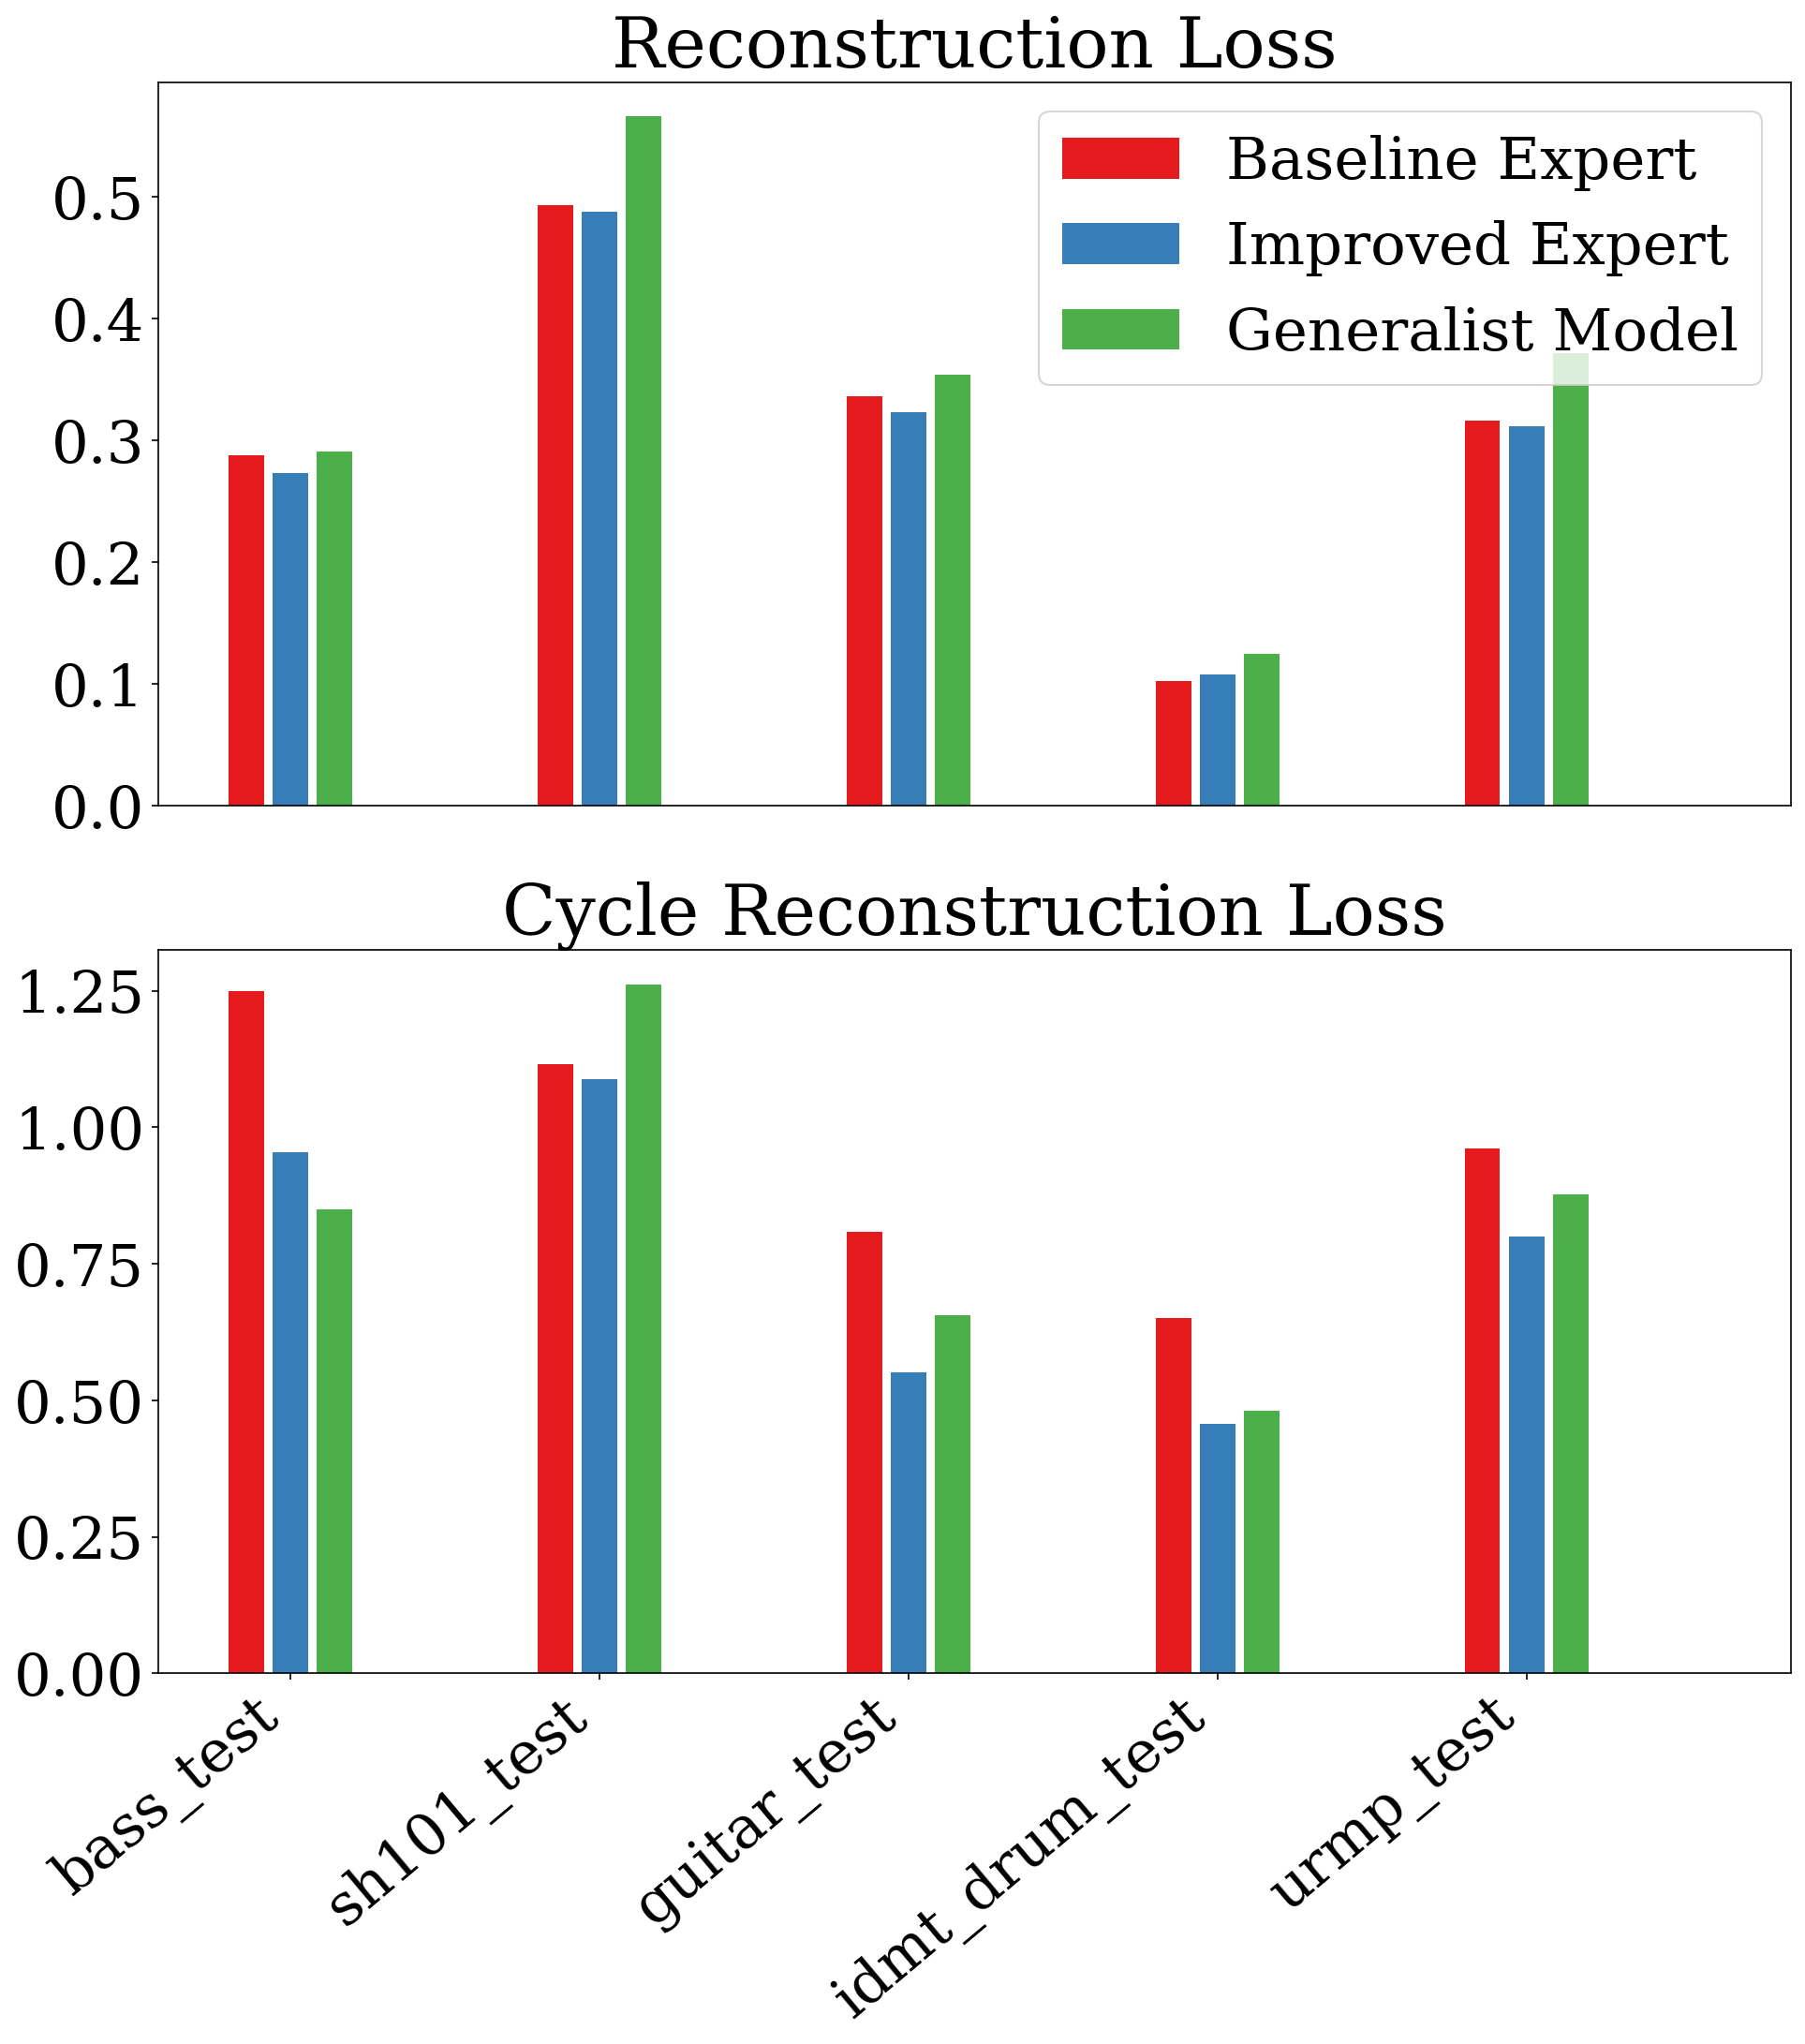
\includegraphics[width=0.7\textwidth]{figures/all_datasets.png}
    \caption{Improved Baseline: Comparison on all datasets}
    \label{fig:multi-datasets}
    \small{For each dataset, three models are compared: two experts (with new and old architecture) that were trained on the corresponding train data set containing similar sounds, and one generalist that was trained on the combined train set. It seems that the generalist model can handle a large number of instruments, but a mixture of experts trained on sounds similar to the target sound still outperforms the generalist model. In some cases, the metrics differ greatly from subjective listening tests: the reconstructions of the improved model on sh101 actually sound good compared to the baseline.}
\end{figure}



\section{Few-Shot Transfer to a New Instrument}
\label{transfer}
In the previous sections, the model learned to perform one-shot timbre transfer for a melody and a timbre audio sample, but with the limitation that the target timbre has to be contained in the train dataset. Other instruments sound unnatural - a reconstruction of a piano sample with the generalist model sounds as if it is somewhat influenced by the sh101 data in the train set. \newline
For this section, I attempt to perform timbre transfer to a piano sample with only one audio sample of 96 seconds length to learn from.
The expert guitar models were trained on only 38:10 minutes of audio data - so the question is whether a pre-trained model can be used to learn from much less data. \newline
A common form of performing transfer learning is to use a pre-trained model that performs well on a related task - such as modeling various other instruments if the new task is modeling a piano - and continue training the model on data of the new task.
Often, the first layers of the pre-trained model remain fixed during this fine-tuning step.
Natural language models such as BERT \citep{bert} add task-specific output heads to the pre-trained model - this is especially required if the target task requires a differently shaped output compared to the pre-trained model. \newline
In the first experiment of this section, the complete model is fine-tuned on the piano sample ("Für Elise").
After every step, reconstruction error and cycle reconstruction error are evaluated on the target timbre - another piano sample, but not the one used for fine-tuning ("Twinkle twinkle little star").
As the cycle-reconstruction loss is the relevant performance measure here, experiments in \Cref{fine-tune-cycle} will integrate this into the training objective. Additional melodies of the train dataset are used as intermediate melodies to compute and minimize the cycle reconstruction loss. \newline
In \Cref{decoder-only}, only the decoder is fine-tuned.
Consider again the idea used in Jukebox, where an autoencoder is used as a part of a larger model. The autoencoder produces a latent code that serves as the ground truth for a sequence model. If a DDSP-based autoencoder were to be used in such a setting, it would be desirable to have a fixed encoder as otherwise, the sequence model would need to adapt to the new latent code. However, an improved decoder can easily be installed in an existing model - so it is desirable to fine-tune only the decoder. \newline
This brings us to the next question: can multitask fine-tuning be used to give the model additional capabilities without compromising performance on the original task? It is possible that if the encoder has not been trained to distinguish between a piano and a guitar, there are some limits to the fine-tuning that can be achieved with the decoder-only approach.\newline
The experiments show that each variant works to some extent - in particular listening tests show that a fine-tuned model can mimic the sound of a piano better. However, the losses do not converge to a much better value than the pretrained model. An overview of the metrics is given in \Cref{fig:tuning-overview}. \newline
One reason for this is that minor errors of the $f_0$ curve cannot be fixed by the model and lead to a large u-MSS error, especially in the upper harmonics, where the pitch difference is multiplied by the harmonic index. As a way to overcome this, I tried using u-MSS with mel-spaced frequency bins. The mel-scale attempts to be a perceptually uniform scale and has a lower frequency resolution in the upper frequencies. The experiments in \Cref{mel-mss}, however, do not solve the issue of fluctuating loss during fine-tuning. \newline



\begin{figure}
    \begin{minipage}[b]{0.45\textwidth}
        \centering
        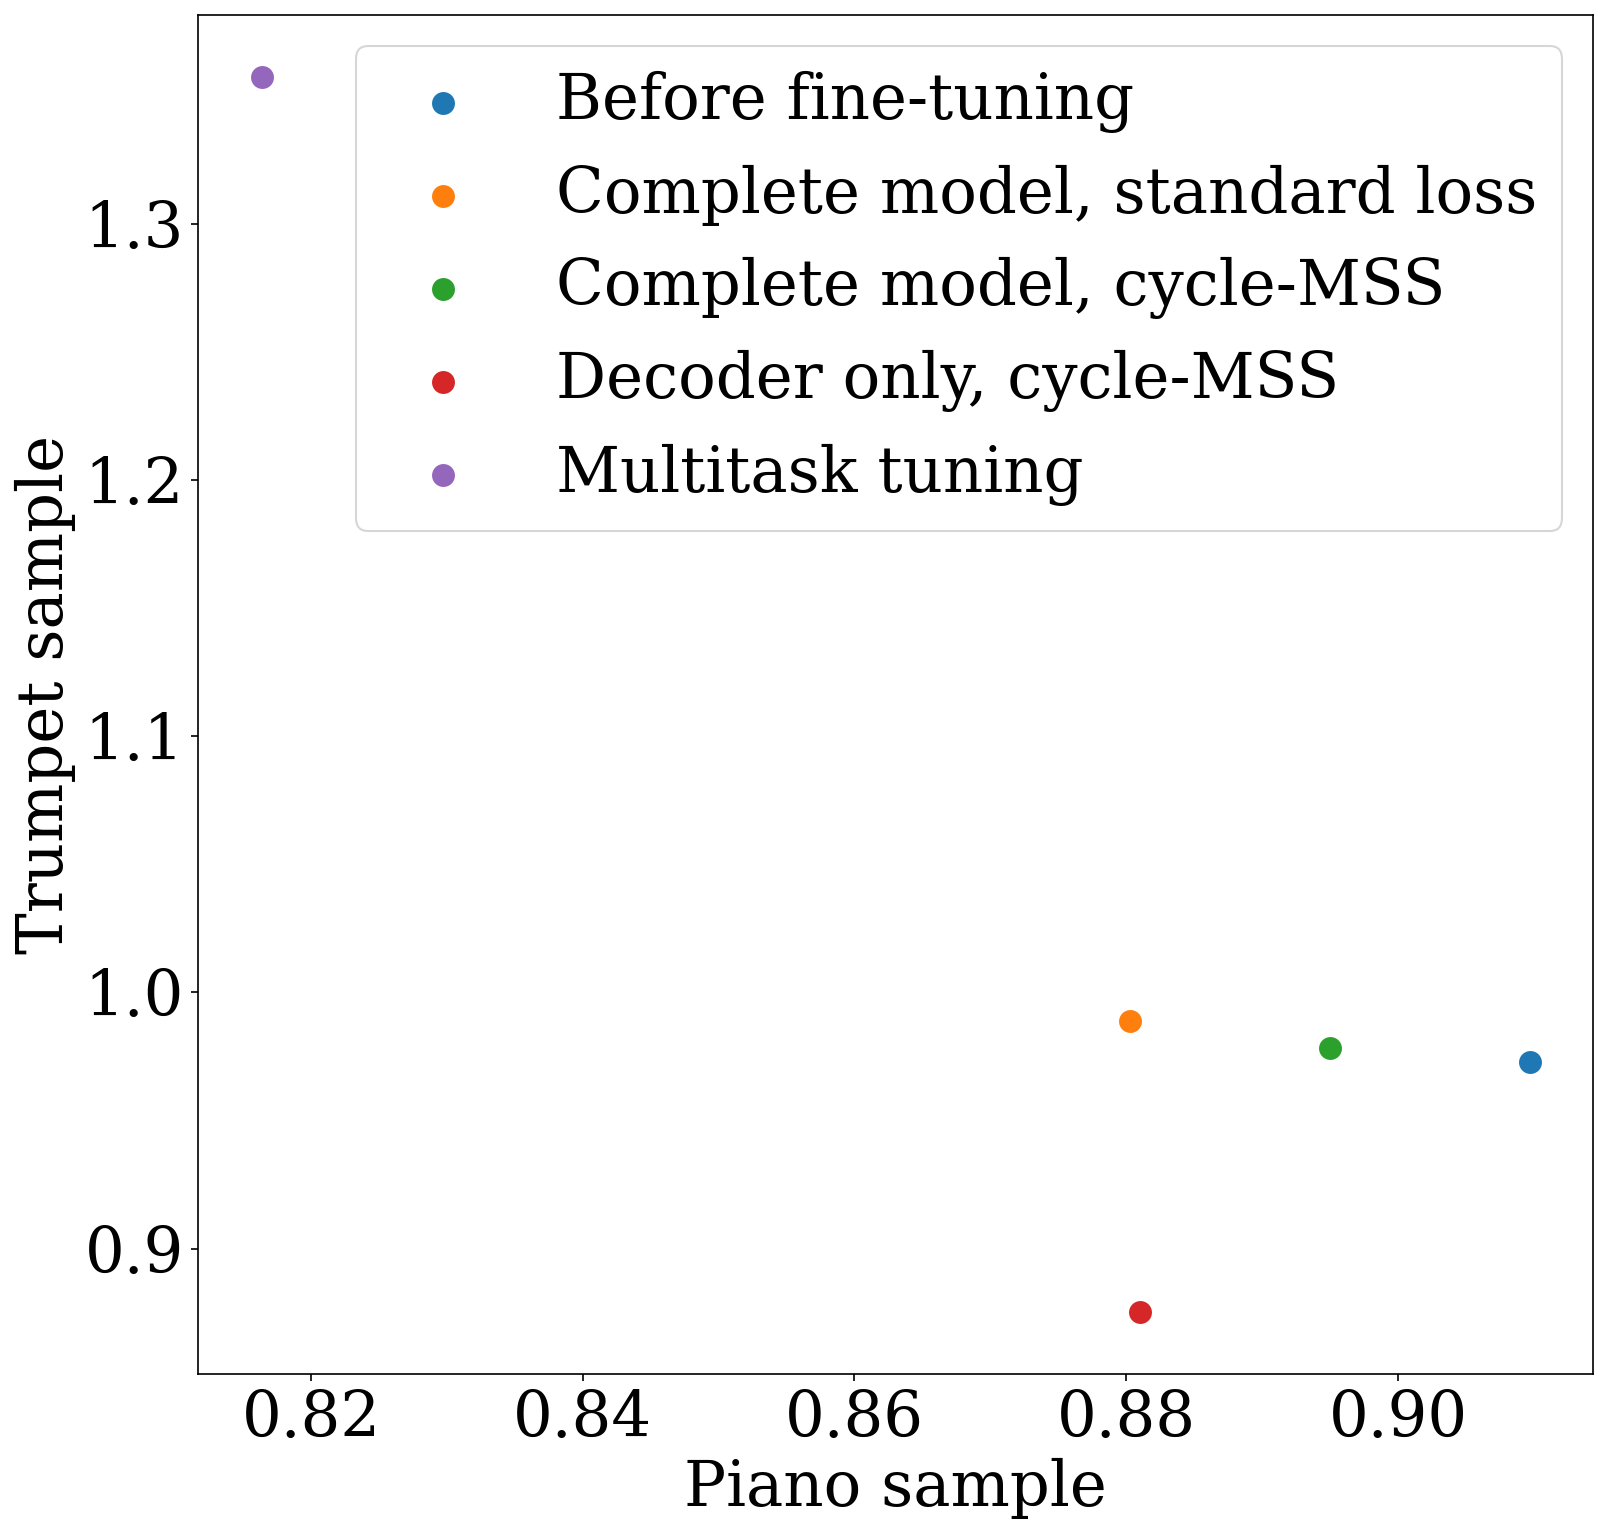
\includegraphics[width=\textwidth]{figures/fine-tuning/overview.png}
        \caption{Metrics for piano and trumpet test sample for all fine-tuning strategies}
        \label{fig:tuning-overview}
        \small{Each variant leads to improved cycle-reconstruction metrics on the test sample, even though it is not the same piano. Surprisingly, the multitask fine-tuned model is the least stable and ends up having the worst performance for the trumpet test sample. The loss does not correspond perfectly to the perceived audio quality.}
    \end{minipage}
    \hfill
    \begin{minipage}[b]{0.45\textwidth}
        \centering
        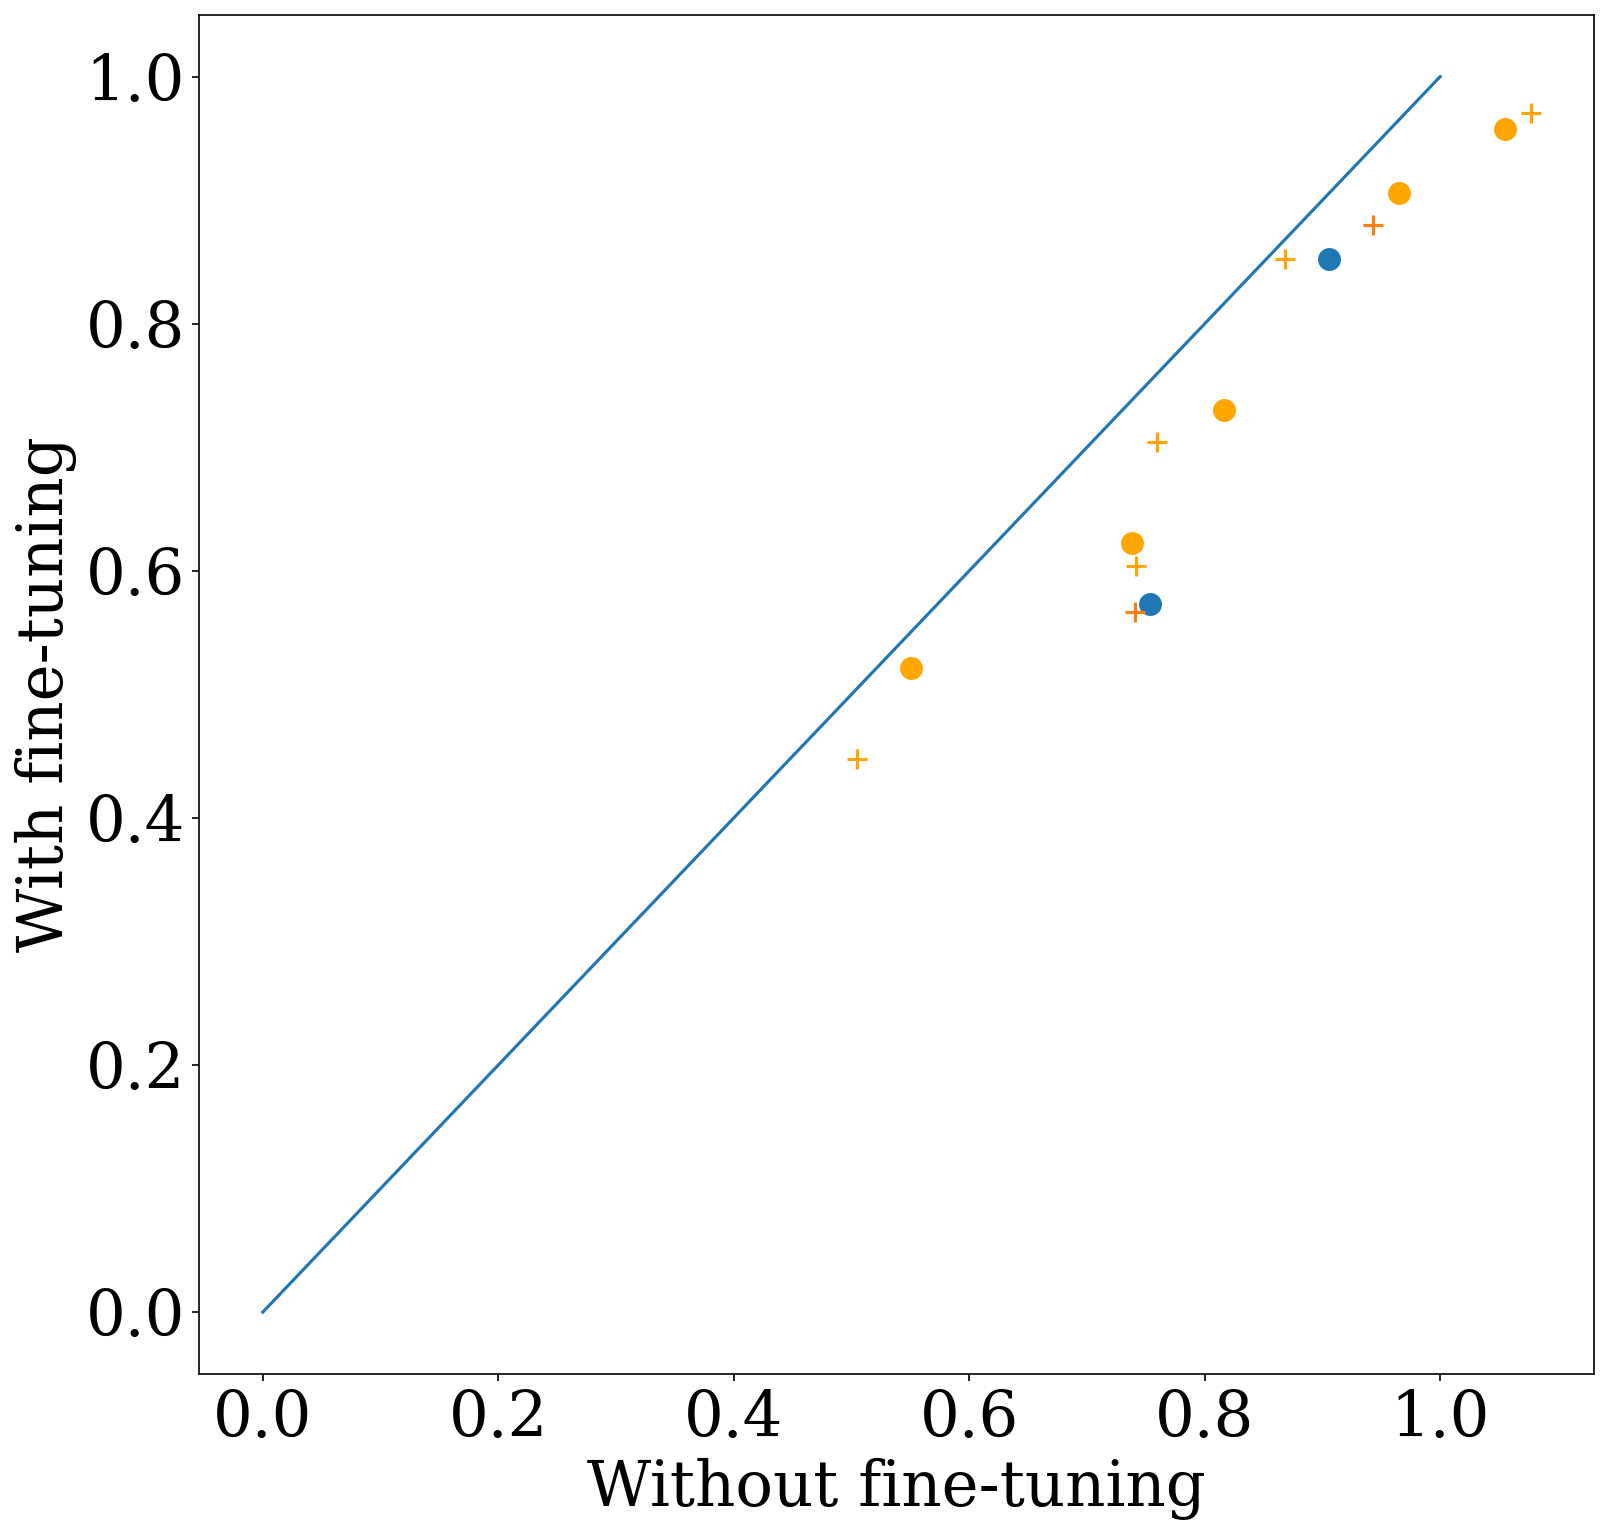
\includegraphics[width=\textwidth]{figures/fine-tuning/final.png}
        \caption{Complete model}
        \small{Here, the loss is compared for various samples of the URMP-test set (orange) and the piano sample (blue). The complete model was fine-tuned on the second half of each test sample individually and evaluated on the first half. Round dots are used for the cycle-reconstruction loss, and the + markers show reconstruction loss.}
    \end{minipage}
    
    
   
\end{figure}

\subsection{Fine-Tuning the Complete Model}
\label{sec:complete-model}
For the first experiment, training of the autoencoder is simply resumed for 100 steps with snippets of the fine-tuning data. The best performance occurs after seven steps of fine-tuning. Indeed, at this point, the cycle reconstruction loss and the reconstruction loss have improved - however, the reconstruction loss is surprisingly higher than the cycle-reconstruction loss.
Subjectively, the synthesized audio sounds very much like a piano - even after only seven steps of fine-tuning. The complete model with fine-tuning can be used to synthesize new melodies with the timbre of any monophonic instrument in \href{https://colab.research.google.com/github/nielsrolf/ddsp/blob/master/ddsp/colab/experiments/inference.ipynb}{this colab notebook}. \newline
A poor property of this approach is the fact that fine-tuning does not seem to converge reliably. Instead, both reconstruction and cycle reconstruction losses are going up and down after the first few iterations. This issue persists during the rest of these experiments. \newline
Considering that the loss on the train sample does go down quite reliably, the larger error on the test sample can also be due to differences between the sound of the two piano samples. This also explains why the loss seems to be much worse on the test sample, even while the audio sounds like a very convincing piano.


\begin{figure}
    \begin{minipage}[b]{0.45\textwidth}
        \centering
        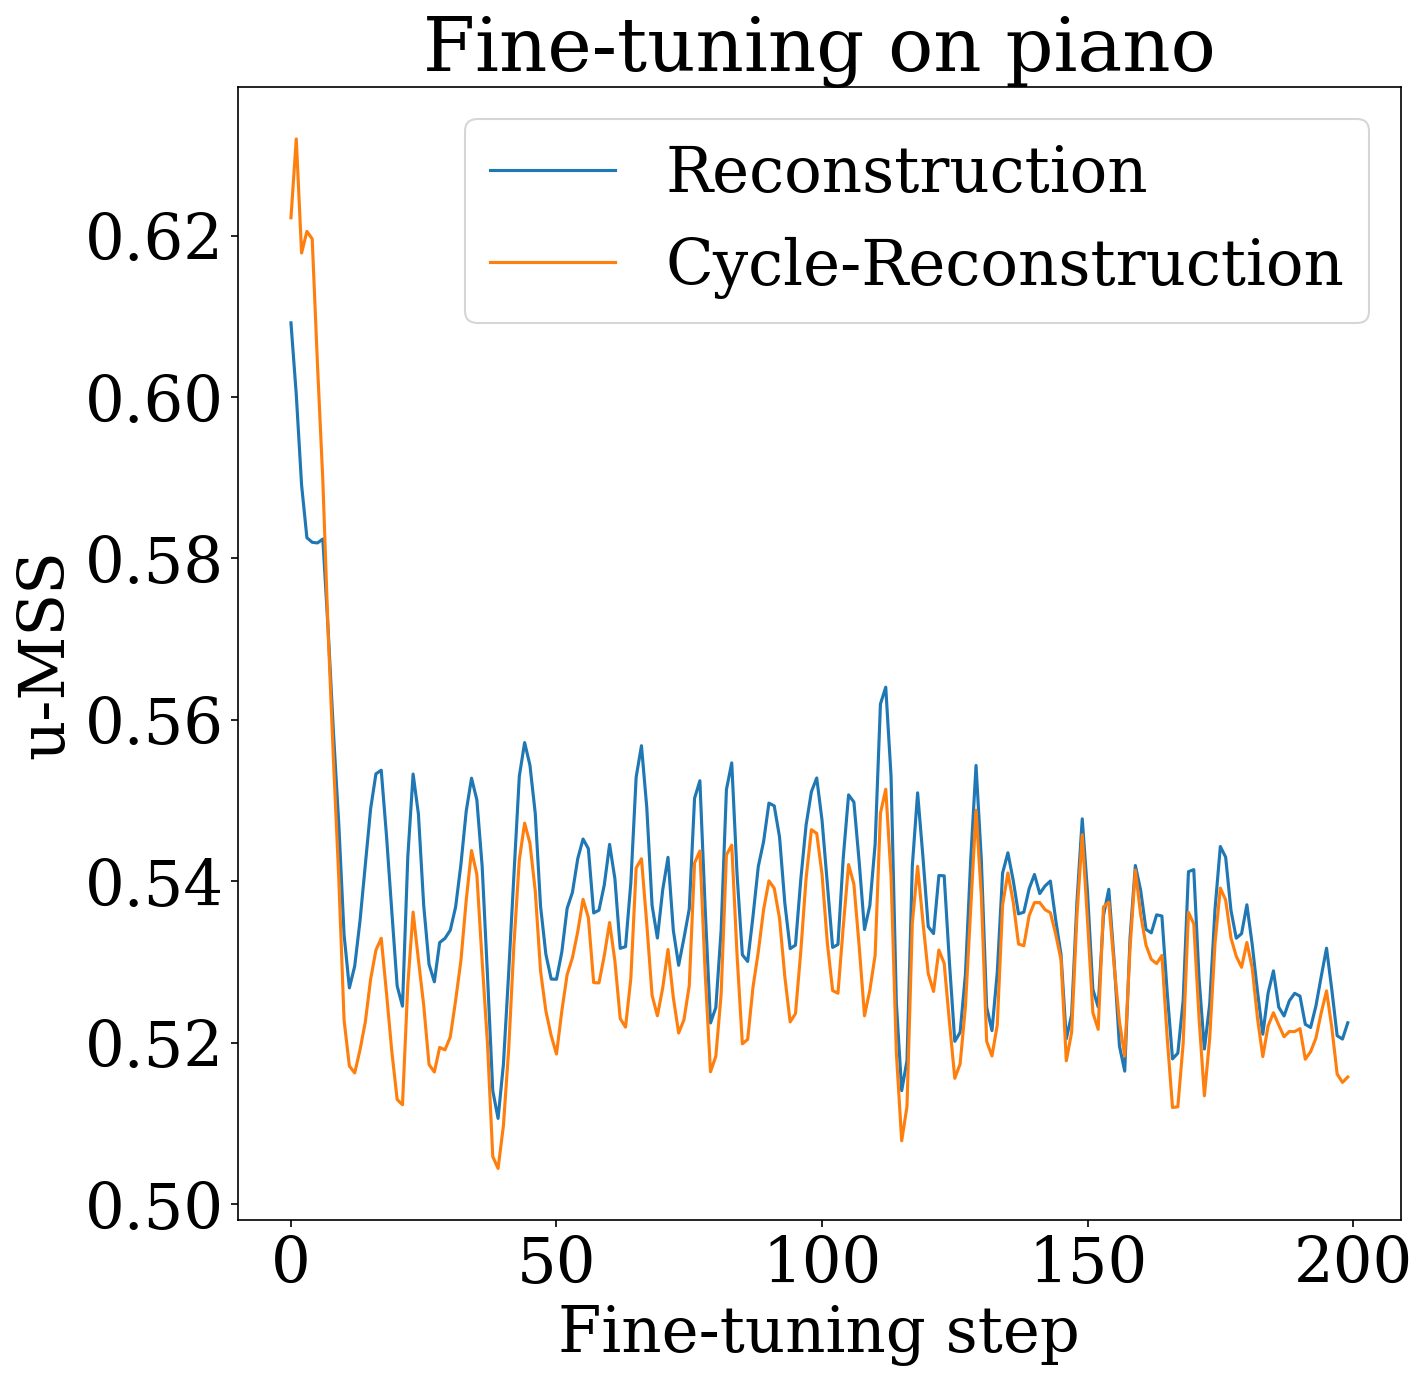
\includegraphics[width=\textwidth]{figures/fine-tuning/exp1/metrics_over_step_train.png}
        \small{\newline Training sample}
    \end{minipage}
    \hfill
    \begin{minipage}[b]{0.45\textwidth}
        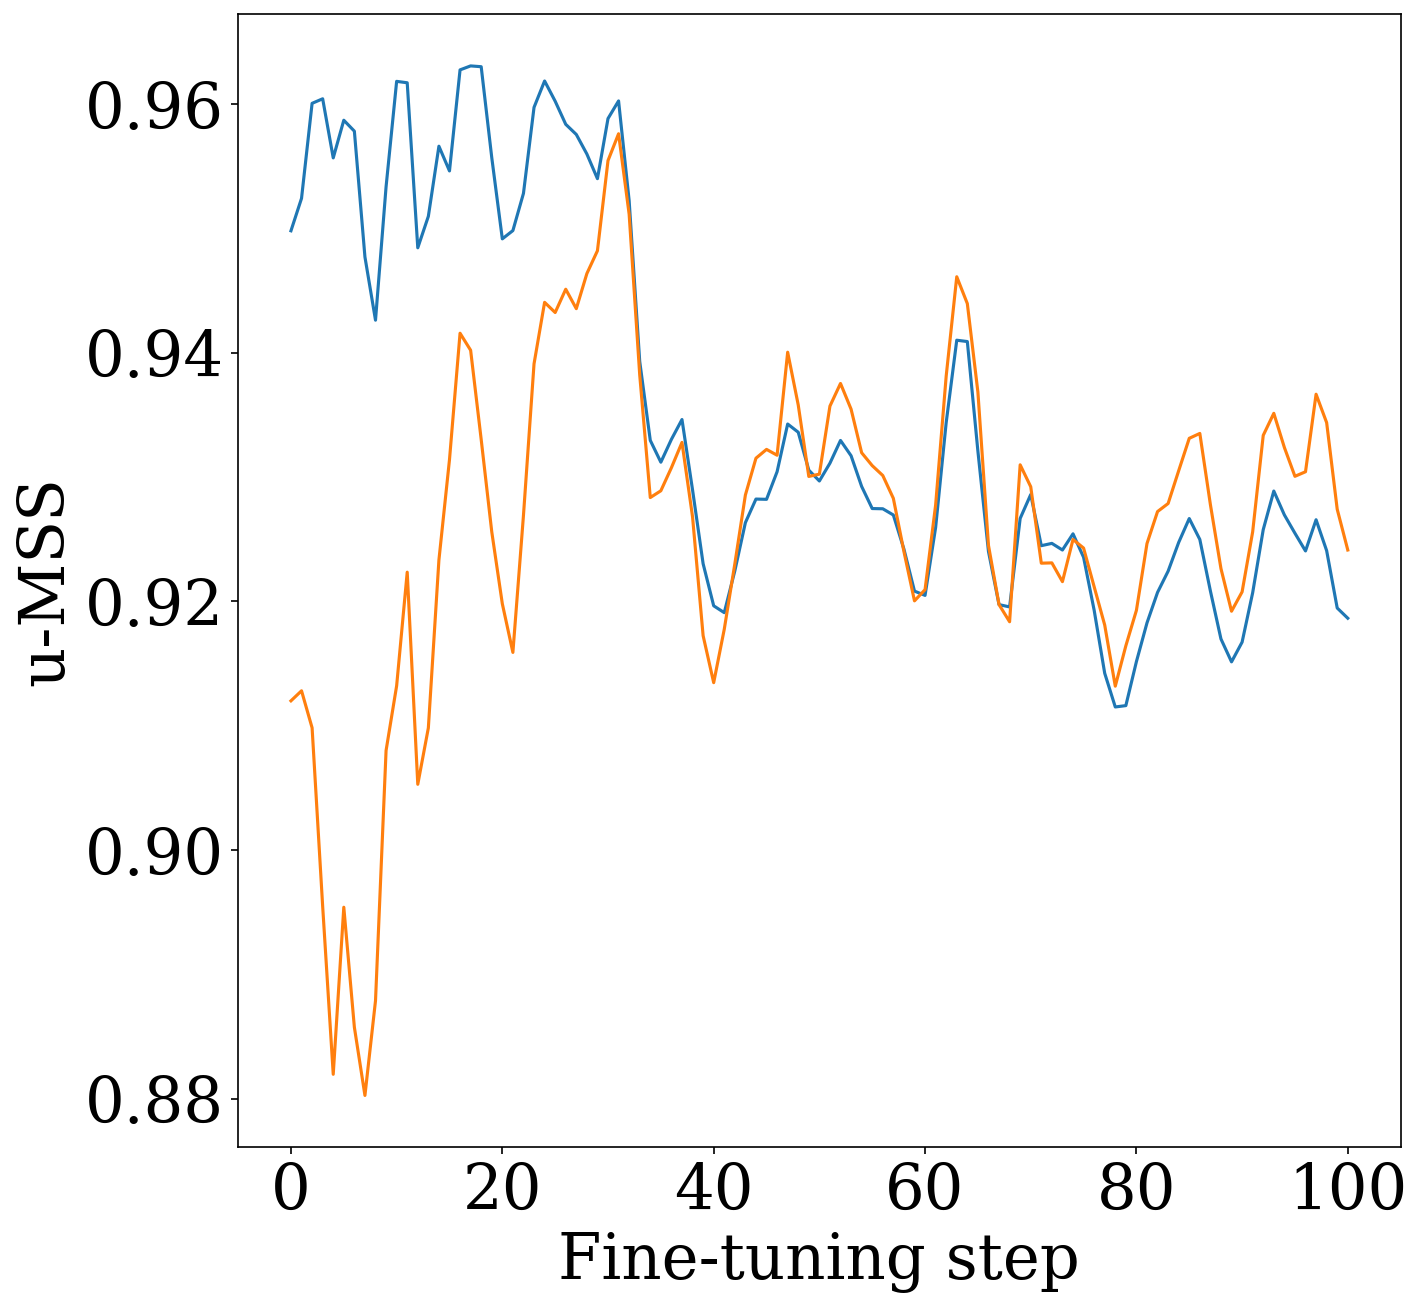
\includegraphics[width=\textwidth]{figures/fine-tuning/exp1/metrics_over_step_twinkle.png}
        \small{\newline Test sample}
        \centering
    \end{minipage}
    \caption{Fine-Tuning the Complete Model}
    \label{fig:fine-tune-complete}
    
\end{figure}

\begin{figure}
    \begin{minipage}[b]{0.45\textwidth}
        \centering
        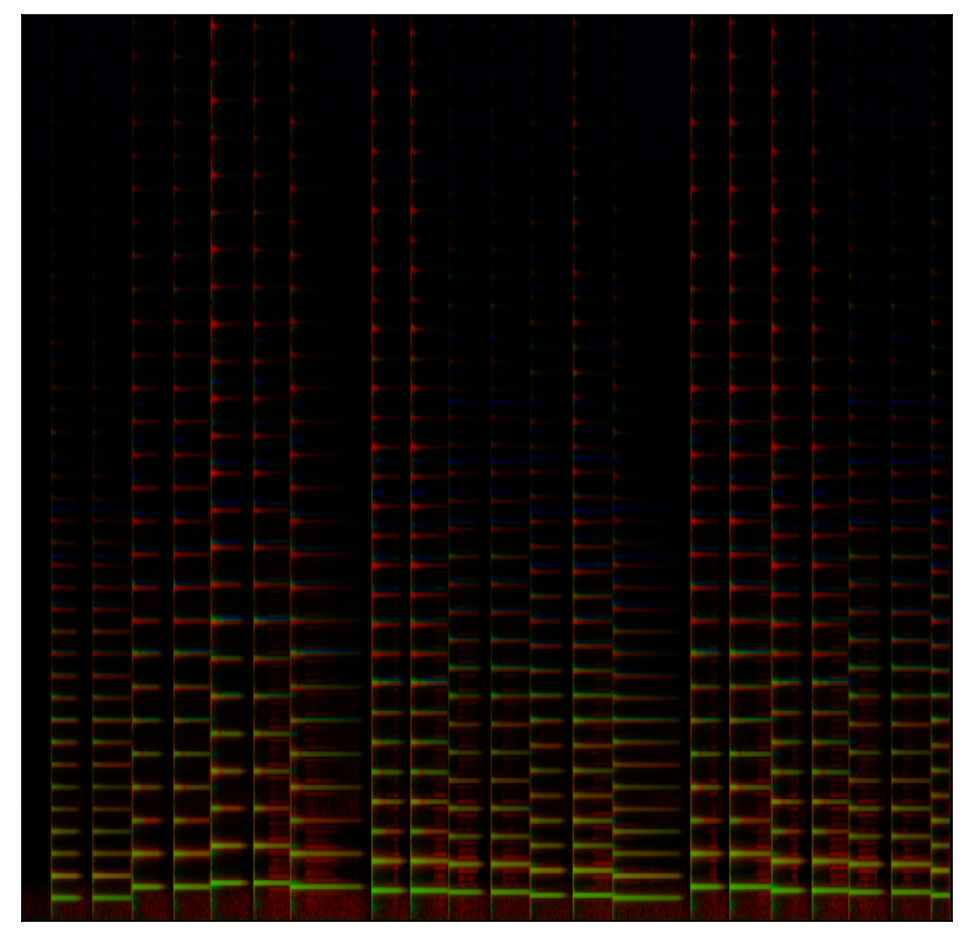
\includegraphics[width=0.8\textwidth]{figures/fine-tuning/twinkle-initial-cycled.png}
        \small{\newline Before fine-tuning}
    \end{minipage}
    \hfill
    \begin{minipage}[b]{0.45\textwidth}
        \centering
        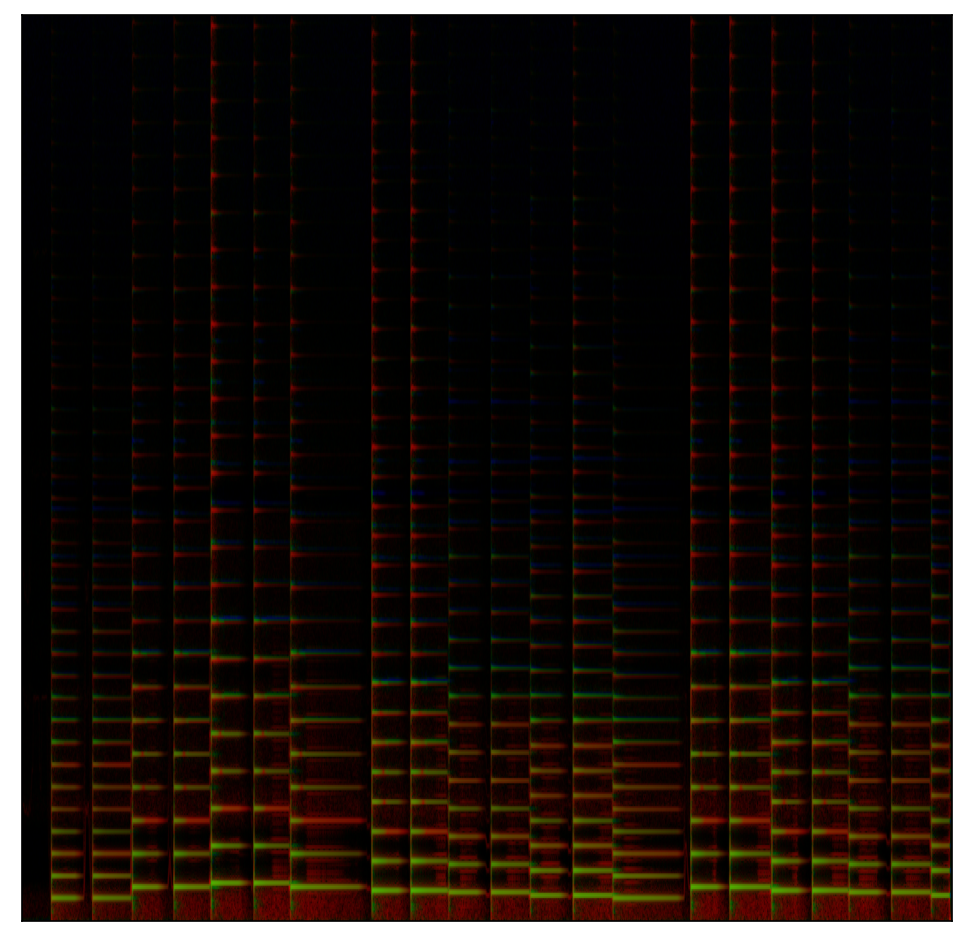
\includegraphics[width=0.8\textwidth]{figures/fine-tuning/exp1/twinkle-cycled-tuned.png}
        \small{\newline After fine-tuning}
    \end{minipage}
    \caption{Cycle reconstruction of a piano sample before and after fine-tuning}
    \label{fig:fine-tune-example-1}
    \small{Even though the heatmaps look similar, a clear difference can be heard between the two reconstructions. After fine-tuning for only seven steps, the audio sounds clearly like a piano.}
\end{figure}



\subsection{Cycle-Reconstruction Loss as Training Objective}
\label{fine-tune-cycle}
In the previous experiments, the cycle reconstruction loss was used as the main performance measure. It is therefore a natural choice to use it also as a training objective.
The complete loss used to train this model is
\begin{equation}
    \begin{split}
    z_x, f_{0,x}, ld_x &= encode(x) \\
    z_y, f_{0,y}, ld_y &= encode(y) \\
    rec &= decode(z_x, f_{0,x}, ld_x ) \\
    transfer &= decode(z_x, f_{0,y}, ld_y ) \\
    \hat{z_{x}}, \hat{f_{0,y}}, \hat{ld_y} &= encode(transfer) \\
    cycled &= decode(\hat{z_{x}}, f_{0,x}, ld_x ) \\
    loss &= MSS(x, rec) + MSS(x, cycled)
    \end{split}
\end{equation}
where $x$ is a sample of the txarget timbre, and $y$ is sound of any intermediate melody - here taken from the combined train set. The best performance is reached after 17 steps of fine-tuning and sounds a bit better than the model trained without cycle-reconstruction loss as objective. It is therefore kept for the following experiments.


\begin{figure}
    \centering
    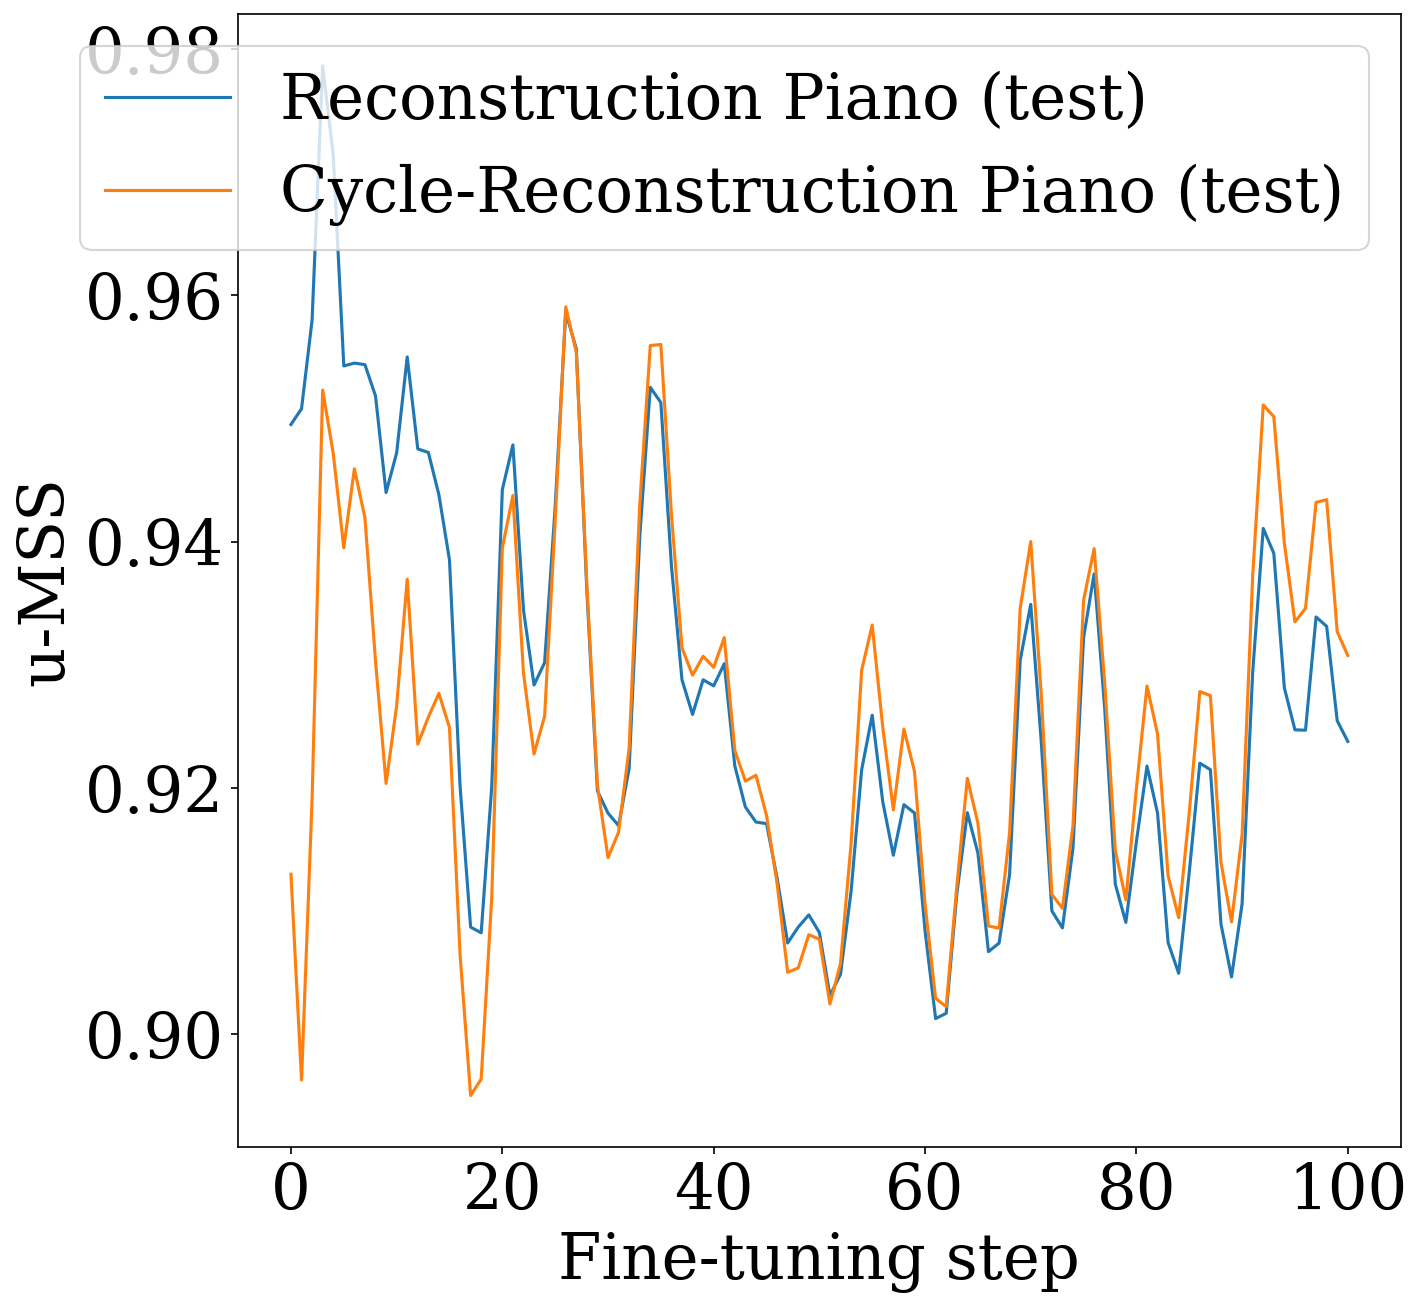
\includegraphics[width=0.5\textwidth]{figures/fine-tuning/cycle-objective/metrics-over-step.png}
    \captionsetup{justification=centering,margin=2cm}
    \caption{Fine-Tuning the Complete Model, Cycle-Reconstruction Loss as Training Objective}
    \label{fig:cycle-loss-objective}
    
\end{figure}


\subsection{Fine-Tuning the Decoder Only}
\label{decoder-only}
In the next experiment, the encoder remains fixed, and the decoder is fine-tuned. Now, in addition to the metrics for the target timbre, consider the performance of the fine-tuned model for a trumpet sample. 
We can observe that the model does not unlearn its ability to model other instruments, but the performance varies in a similar way as the performance on the piano. \newline
The overall sound quality is not significantly improved, and the minimal loss is reached after two steps of fine-tuning already.

\subsection{Multitask Fine-Tuning}
\label{fine-tune-multitask}

\begin{figure}
    \begin{minipage}[b]{0.45\textwidth}
        \centering
        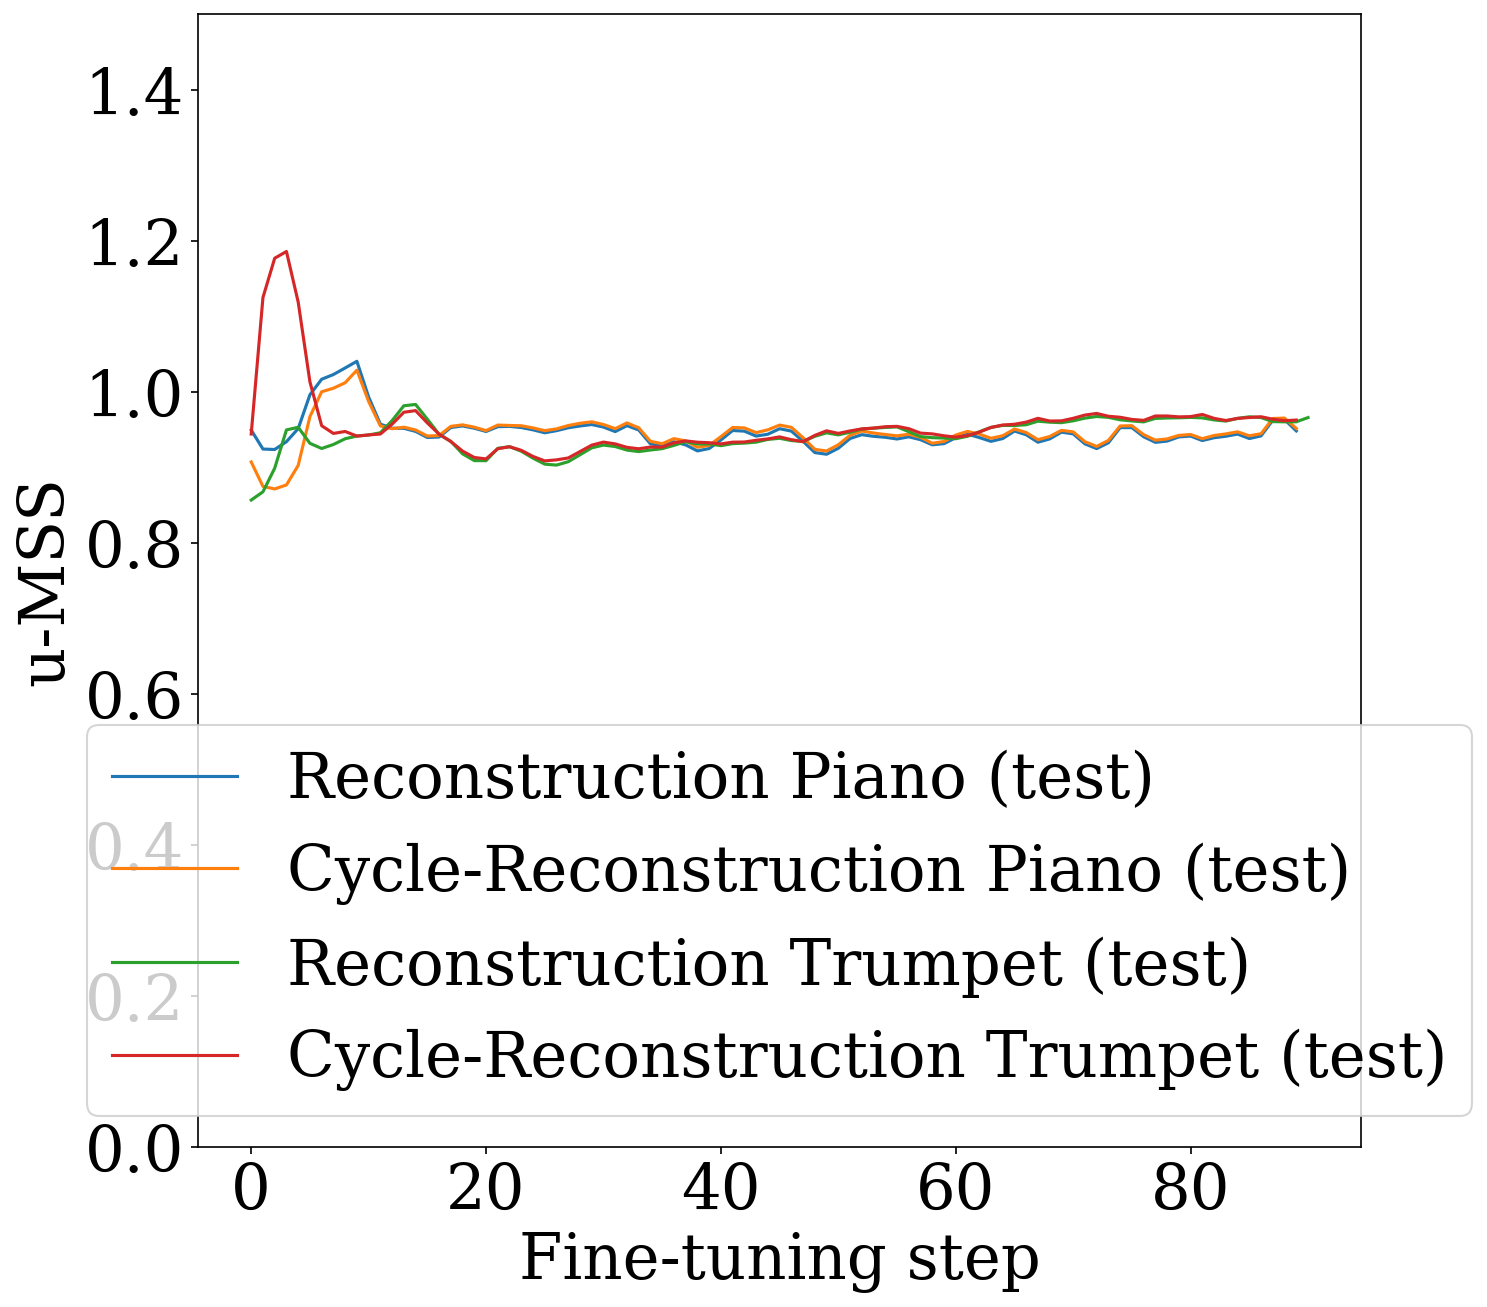
\includegraphics[width=\textwidth]{figures/fine-tuning/decoder-only/metrics-over-steps.png}
        \small{\newline Only piano}
    \end{minipage}
    \hfill
    \begin{minipage}[b]{0.45\textwidth}
        \centering
        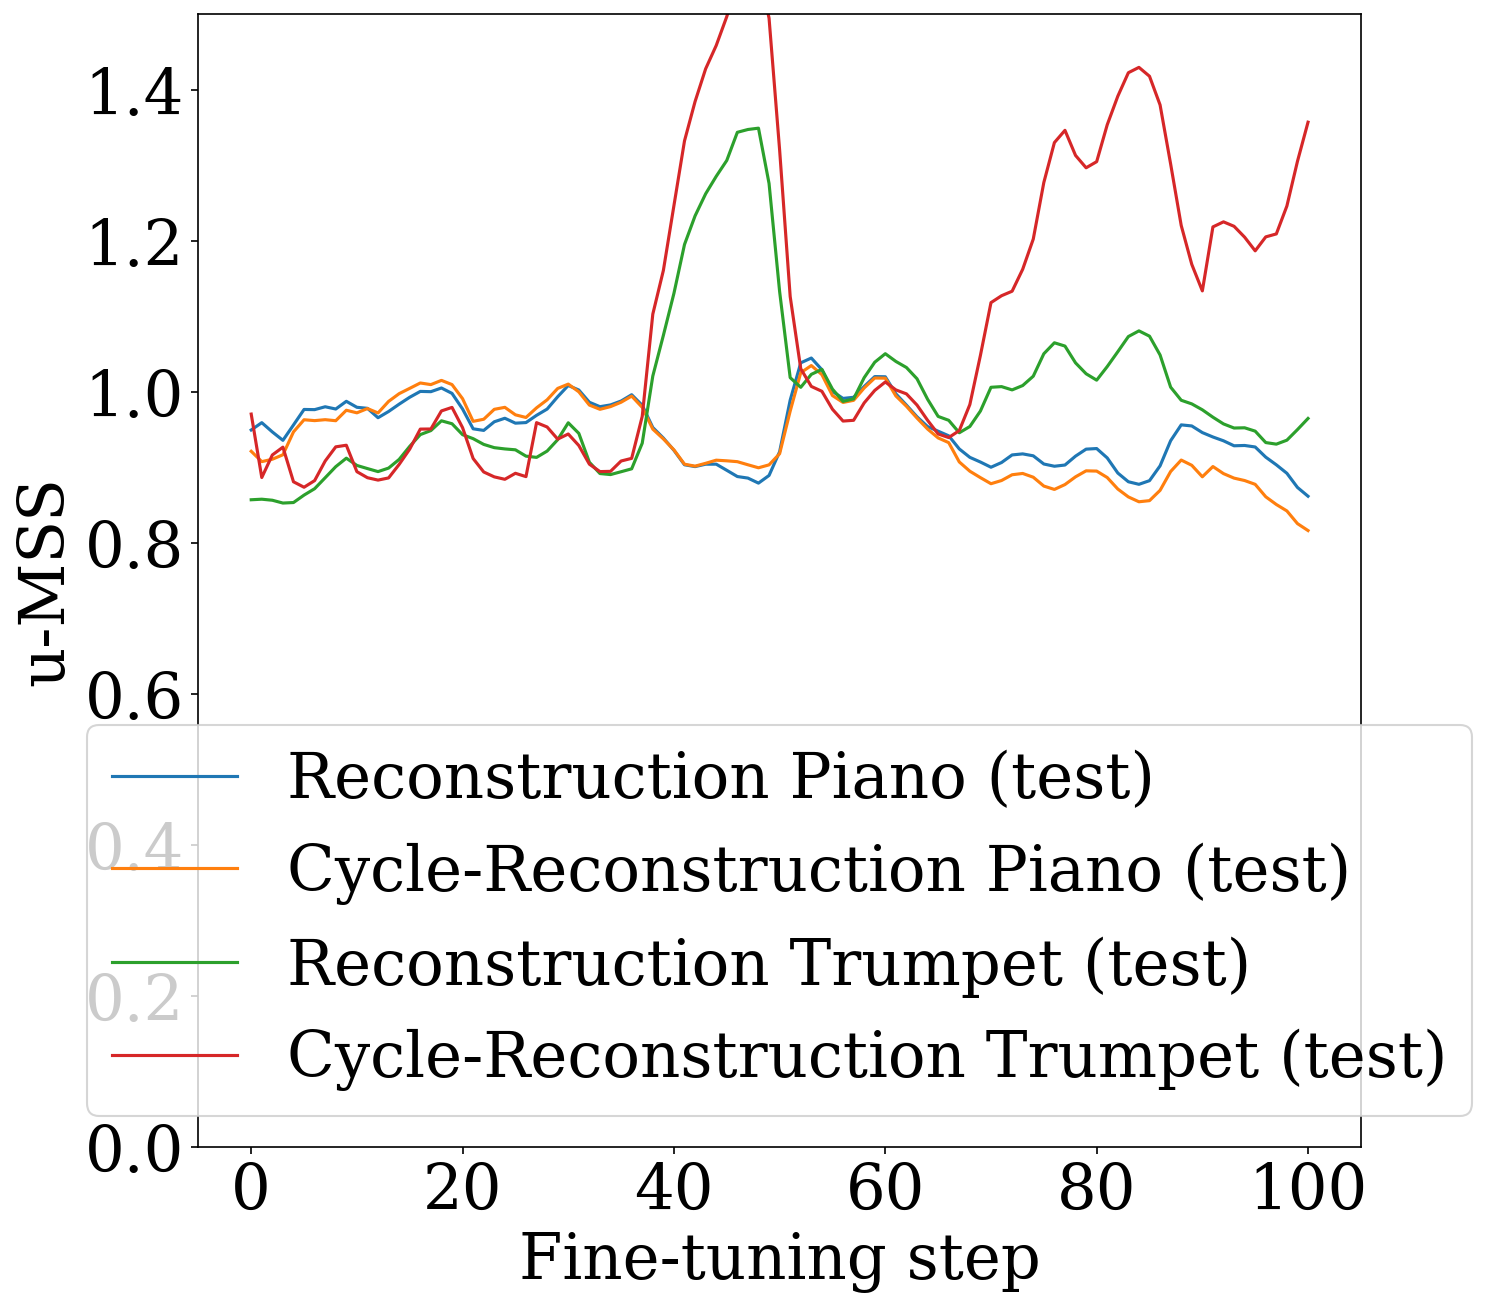
\includegraphics[width=\textwidth]{figures/fine-tuning/multi-task/metrics.png}
        \small{\newline Piano + combined train}
    \end{minipage}
    \caption{Fine-Tuning the Decoder, single task vs multitask}
    \label{fig:decoder-only}
\end{figure}
In the previous experiments, the model did not unlearn to model other instruments to a large degree. This suggests we can even fine-tune it on the original training data and the new data combined. For this experiment, exactly the same setup as in the previous setup has been used  with the only change, that now only two out of four samples in the batch are of the piano, while the other two samples are taken from the combined train set. \newline
As can be seen in \Cref{fig:decoder-only}, the model behaves in unexpected ways during training. The best cycle-reconstruction loss is reached at the very end of the 100 steps of training, but it sounds worse than samples generated in the previous experiments. For potential use cases, this means that rather than continuously fine-tuning a model on more and more instruments, it is better to adapt the model each time it is used for an instrument that the pretrained autoencoder does not handle sufficiently well. Due to the small number of update steps required to fine-tune the model, fine-tuning and inference combined can still be done in a matter of minutes.


\subsection{Mel-MSS}
\label{mel-mss}

If we look closely at the error heat maps for a reconstruction of the test sample, we can see that there are many small errors at the high frequencies, simply because $f_0$ seems to be slightly off.
This can be observed in \Cref{fig:mel-mss} in the form of red areas with a blue area above them.
Since the $f_0$ extraction is not learned by the autoencoder, we do not necessarily want to penalize this type of error. 
This motivates the use of mel-spaced spectrograms for computing the MSS, which don't suffer from this problem due to their lower frequency resolution. Fine-tuning with this objective, however, does not lead to a better convergence, as \Cref{fig:tuning-mel} shows. Fine-tuning was otherwise done as in \Cref{sec:complete-model} - i.e. the complete model was trained including the encoder, and no cycle-reconstruction loss or multitask fine-tuning was used. The resulting audios sound similar to the variant without mel-spectrograms. Therefore this approach does not add to the final performance and hence has been discarded.

\begin{figure}
    \begin{minipage}[b]{0.49\textwidth}
        \centering
        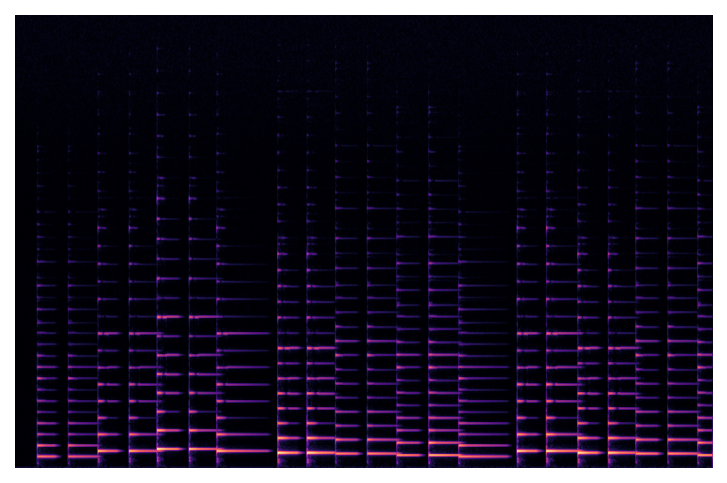
\includegraphics[width=\textwidth]{figures/fine-tuning/mel/spec.png}
        \small{\newline Spectrogram}
        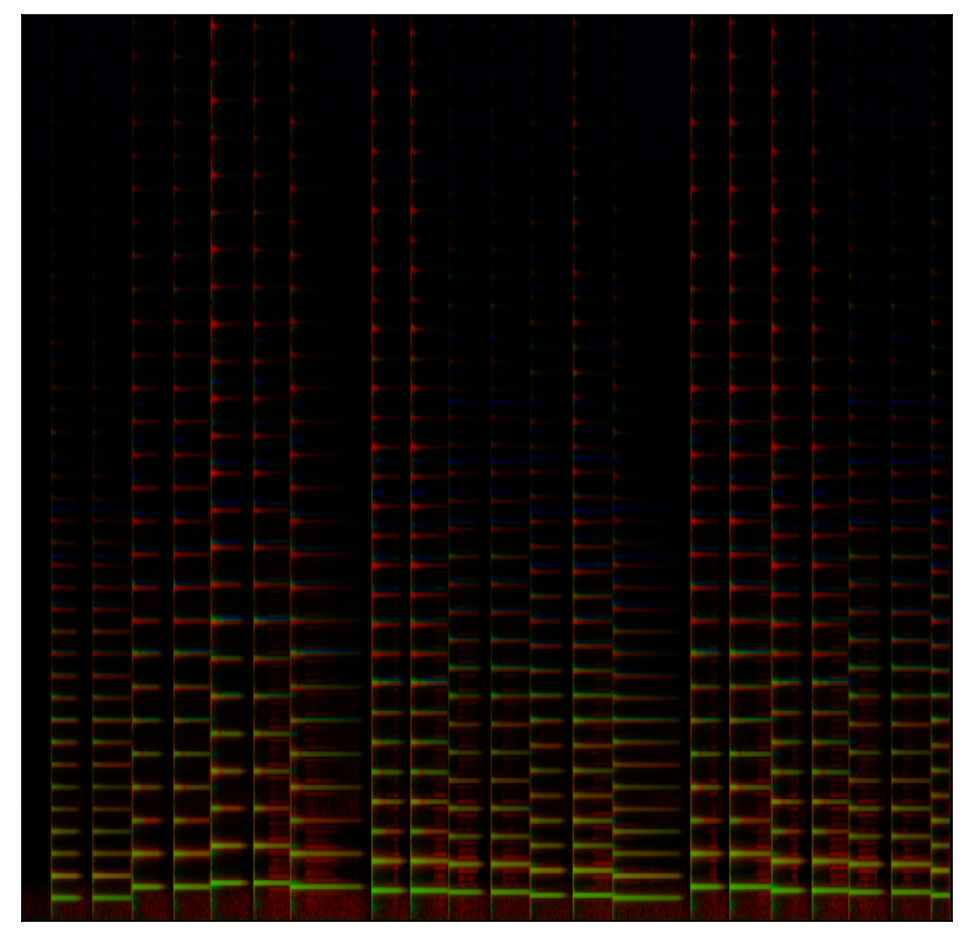
\includegraphics[width=\textwidth]{figures/mss/piano-untuned-cycled.png}
        \small{\newline Spectrogram Error}
    \end{minipage}
    \hfill
    \begin{minipage}[b]{0.49\textwidth}
        \centering
        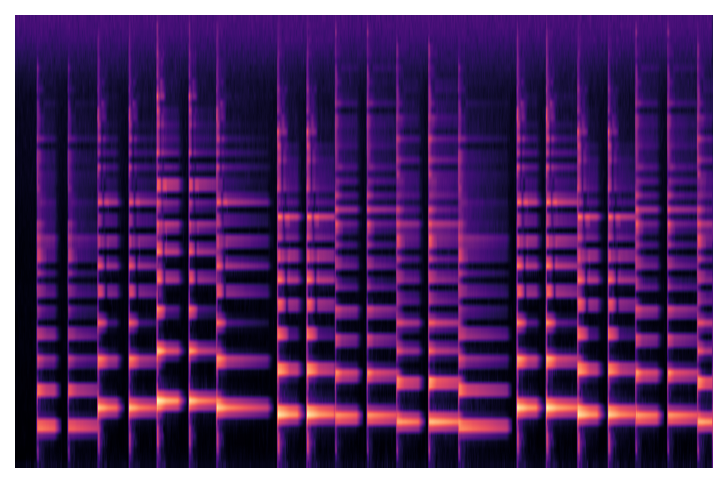
\includegraphics[width=\textwidth]{figures/fine-tuning/mel/melspec.png}
        \small{\newline Mel-Spectrogram}
        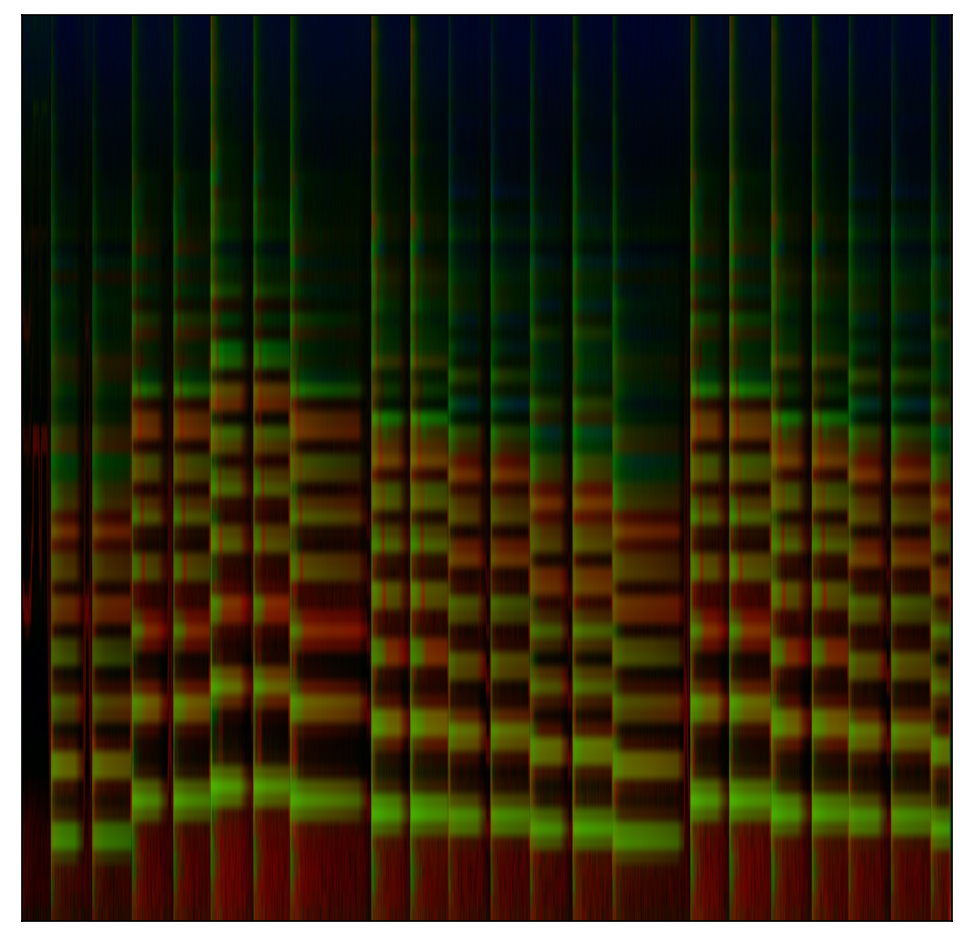
\includegraphics[width=\textwidth]{figures/mss/mel-piano-untuned-cycled.png}
        \small{\newline Mel-Spectrogram Error}
    \end{minipage}
    \caption{Mel-Spectrogram Error}
    \small{A mel-spectrogram has a lower frequency resolution in the upper part, allowing for minimal errors of the predicted $f_0$-curve. This motivates to use them in the multi-scale spectrogram loss.}
    \label{fig:mel-mss}
\end{figure}


\begin{figure}
    \centering
    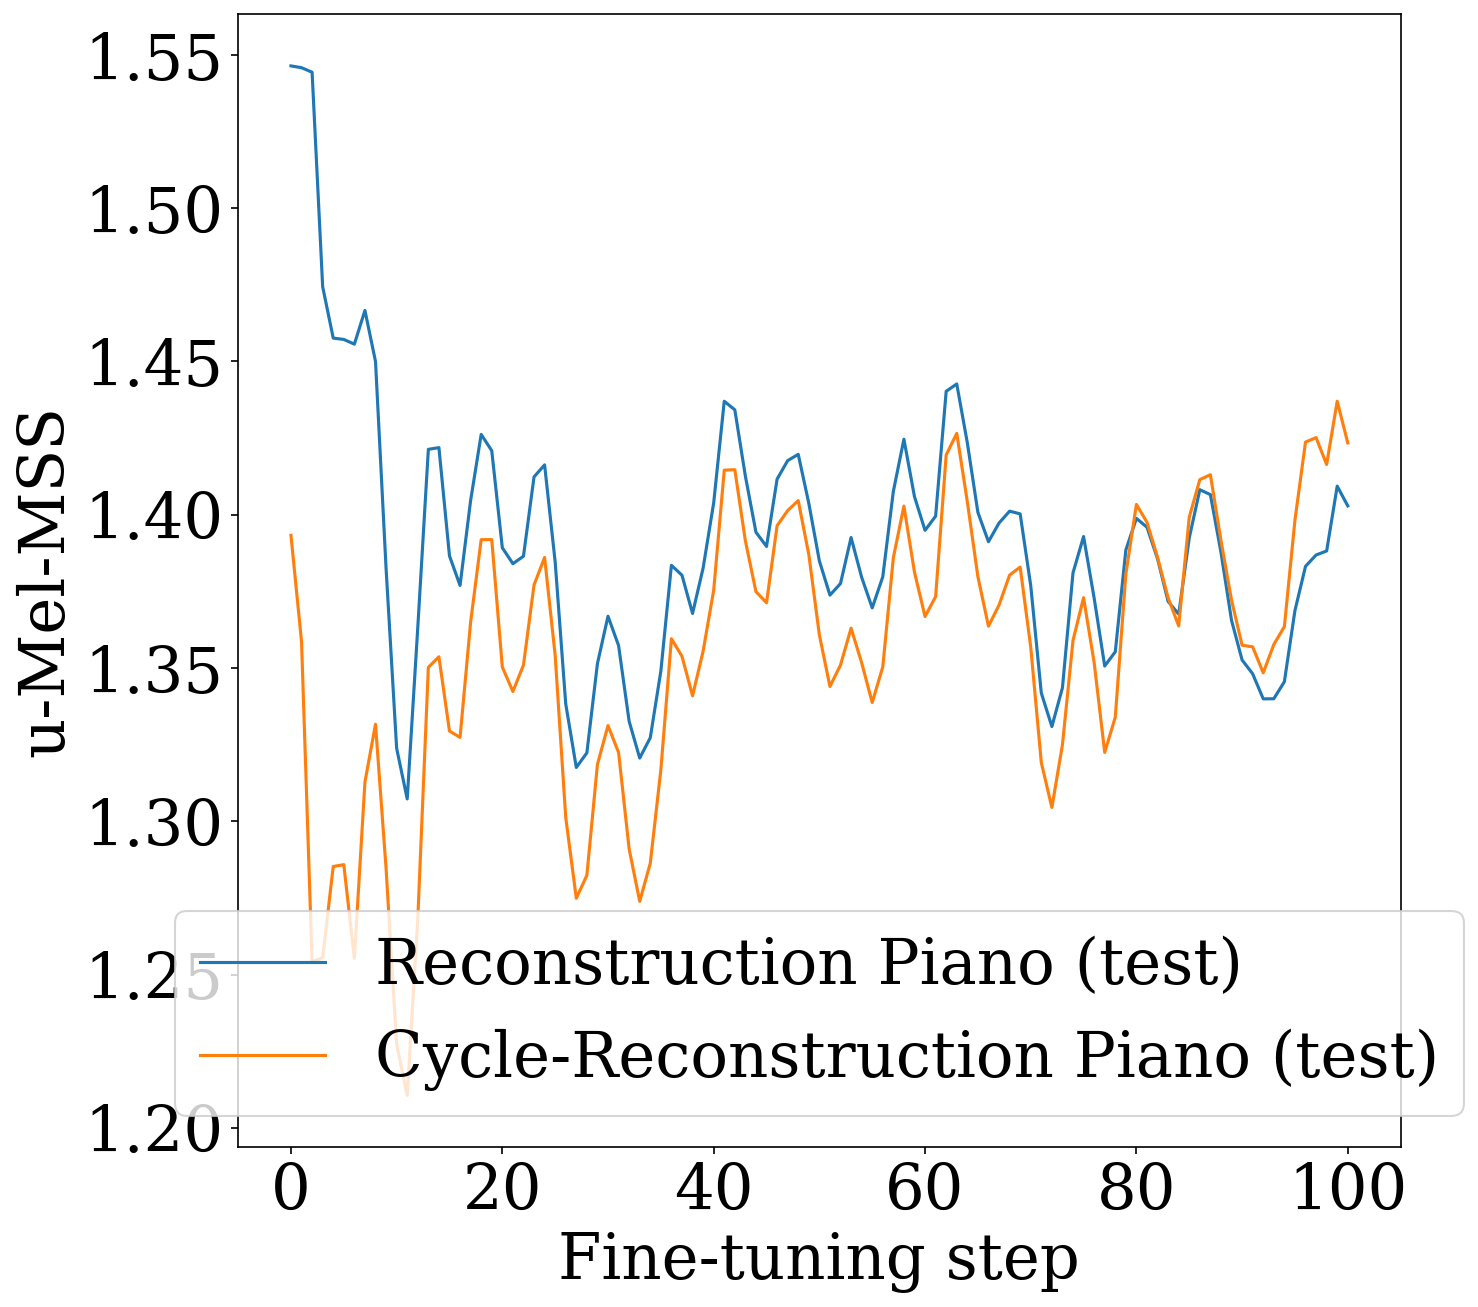
\includegraphics[width=0.5\textwidth]{figures/fine-tuning/mel/metrics.png}
\caption{Fine-Tuning with mel-MSS}
\label{fig:tuning-mel}
\end{figure}

% comparison plot